%!TEX root = ../thesis.tex
%*******************************************************************************
%*********************************** First Chapter *****************************
%*******************************************************************************
\chapter{Uncertainty quantification in computer experiments}
%*******************************************************************************
\hfill
\localtableofcontents
\newpage

%============================================================%
%============================================================%
\section{Introduction}\label{sec:}
%============================================================%
%============================================================%

The progress of computer simulation gradually allows the virtual resolution of more complex problems in scientific fields such as physics, astrophysics, engineering, climatology, chemistry, or biology.
This domain often provides a deterministic solution to complex problems depending on several inputs. 
Associating a UQ analysis with these possibly nonlinear numerical models is a key element to improving the understanding of the phenomena studied. 
A wide panel of UQ methods has been developed over the years to pursue these studies with a reasonable computational cost. 

This chapter presents the standard tools and methods from the generic UQ framework \elias{add ref to intro}, exploited later in this thesis. 
It is structured as follows: Section \elias{add ref} describes the context of the model specification step; 
Section \elias{add ref} presents a classification of the inputs uncertainties and the probabilistic framework to model them; 
Section \elias{add ref} and xx introduce various methods to propagate the input uncertainties through the numerical model for different purposes;
finally, Section \elias{add ref} presents the main inverse methods to perform sensitivity analysis in our framework.


%============================================================%
%============================================================%
\section{Black-box model specification}
%============================================================%
%============================================================%
The uncertainty quantification studies in our framework are performed around an input-output numerical simulation model. 
This numerical model, or code, is hereafter considered as \textit{black-box} since the knowledge of the underlying physics doesn't inform the UQ methods. 
Alternatively, one could consider \textit{intrusive} UQ methods, introducing uncertainties within the resolution of computer simulation (see e.g., \elias{add ref}).
In practice, the numerical model might be a sequence of codes executed in series to obtain a variable of interest.

Moreover, the simulation model is in most cases deterministic, otherwise, it is qualified as intrinsically stochastic (i.e., two runs of the same model taking the same inputs return different outputs).
Then, most numerical simulation presents modeling errors. 
In the following, it will be assumed that the numerical models passed a \textit{validation \& verification} phase, to quantify their confidence and predictive accuracy. 

Formally, part of the problem specification is the definition of the set of $d$ input variables $\bx = \left(x_1, \dots, x_d\right)\TT$ considered uncertain (e.g., wind speed, wave period, etc.). 
In this thesis, the models considered will only present scalar outputs. 
UQ methods dedicated to other types of outputs exist (see e.g., for time series outputs \citet{lataniotis_2019}, \elias{functional Alvaro?}). 
Let us then define the following numerical model:
\begin{equation}
\iM : \bigg|
    \begin{array}{rcl}
        \iD_{\bx} \subseteq \R^d & \longrightarrow & \iD_{\by} \subseteq \R \\
        \bx & \longmapsto & y.
    \end{array}
\end{equation}

Unlike the typical machine learning input-output dataset framework, the UQ analyst can simulate the output image of any inputs (in the input domain), using the numerical model. 
However, numerical simulations often come with an important computational cost. 
Therefore UQ methods should be efficient and require as few simulations as possible. 
In this context, metamodels (or surrogate models) are statistical approximations of the costly numerical model, that can be used to perform tractable UQ. 
Metamodels are only built and validated on a limited number of simulations (in a \textit{supervised learning} framework).
In practice, the model specification step is often associated with the development of a \textit{wrapper} of the code \elias{explain wrapper}, with can be deployed on a \textit{high-perfomance computer}.
Once the model is specified, a critical step of uncertainty quantification is enumerating the input uncertainties and building an associated mathematical model.


%============================================================%
%============================================================%
\section{Enumerating and modeling the uncertain inputs}
%============================================================%
%============================================================%

%------------------------------------------------------------%
\subsection{Sources of the input uncertainties}
%------------------------------------------------------------%

To ensure a complete risk assessment (e.g., associated with the exploitation of a wind turbine throughout its life span), the analyst should construct a list of uncertain inputs as exhaustive as possible. 
Even if these uncertainties might have different origins, they should all be considered jointly in the UQ study. 
The authors proposed to classify them for practical purposes into two groups:
\begin{itemize}
    \item \textbf{aleatory uncertainty} regroups the uncertainties that arise from natural randomness (e.g., \elias{add example}). 
    From a risk management point of view, these uncertainties are qualified as \textit{irreducible} since the industrials facing them will not be able to acquire additional information to reduce them (e.g., additional measures).     
    \item \textbf{epistemic uncertainty} gathers the uncertainties resulting from a lack of knowledge. 
    Contrarily to the aleatory ones, epistemic uncertainties might be reduced by investigating their origin. 
\end{itemize} 

\citet{kiureghian_2009} offers a discussion on the relevance of this classification. 
They affirm that this split is practical for decision-makers to identify possible ways to reduce their uncertainties. 
However, this distinction should not affect the way of modeling or propagating uncertainties. 
\elias{To illustrate the limits of this split, some uncertainties present both an aleatory and epistemic aspect.}
In the following, the probabilistic framework is introduced to deal with uncertainties. 


%------------------------------------------------------------%
\subsection{Modeling uncertain inputs with the probabilistic framework}
%------------------------------------------------------------%

Uncertainties are traditionally modeled with objects from the probability theory.
In this thesis, the \textit{probabilistic framework} is adopted. 
Alternative theories exist to mathematically model uncertainties. 
For example, imprecise probability theory allows more general modeling of the uncertainties. 
It becomes useful when dealing with very limited and possibly contradictory information (e.g., expert elicitation). 
The core probabilistic tools and objects are introduced hereafter. 

The \textit{probability space} (i.e., a measure space with its total measure summing to one), also called probability triple and denoted $(\Omega, \iA, \mu)$.
This mathematical concept first includes a sample space $\Omega$, which contains a set of outcomes $\omega \in \Omega$. 
An \textit{event} is defined as a set of outcomes in the sample space.
Then, a $\sigma$-algebra $\iA$ (also called event space) is a set of events. 
Finally, a probability function $\mu: \iA \rightarrow [0, 1]$, is a positive probability measure associated with an event.
Most often, the choice of the probability space will not be specified. 
The main object will be functions defined over this probability space: random variables. 

The \textit{random vector} $\bX$ (i.e., multivariate random variable) is a measurable function defined as: 
\begin{equation}
\bX : \bigg|
\begin{array}{rcl}
    \Omega & \longrightarrow & \iD_{\bx} \subseteq \R^d\\
    \omega & \longmapsto & \bX(\omega) = \bx.
\end{array}
\end{equation}
In the following, the random vector $\bX$ will be considered to be a squared-integrable function against the measure $\mu$ (i.e., $\int_{\Omega} |\bX(\omega)|^2 \,\dd \mu(\omega) < \infty$).
Moreover, this work will focus on continuous random variables.

The \textit{probability distribution} of the random vector $\bX$ is the pushforward measure of $\mu$ by $\bX$.
Which is a probability measure on $(\iD_{\bx}, \iA)$, denoted $\mu_{\bX}$ and defined by: 
\begin{equation}
    \mu_{\bX}(B) = \mu(\bX \in B) = \mu(\omega \in \Omega : \bX(\omega)\in B), \quad \forall B \in \iA.
\end{equation}
The \textit{cumulative distribution function} (CDF) is a common tool to manipulate random variables. 
It is a function $F_{\bX} : \iD_{\bx} \rightarrow [0, 1]$ defined for all $\bx \in \iD_{\bx}$ as: 
\begin{equation}
    F_{\bX}(\bx) = \mu(\bX \leq \bx)
            = \mu(X_1 \leq x_1, \dots, X_d \leq x_d)
            = \mu_{\bX}(]-\infty, x_1] \times \dots \times ]-\infty, x_d]).
\end{equation}
The CDF is a positive, increasing, right-continuous function, which tends to $0$ as $\bx$ tends to $-\infty$ and to $1$ as $\bx$ tends to $+\infty$.
In the continuous case, one can also define a corresponding \textit{probability density function} (PDF) $f_{\bX}: \iD_{\bx} \rightarrow \R_+$  with 
$f_{\bX}(\bx) = \frac{\partial^d F_{\bX}(\bx)}{\partial x_1 \dots \partial x_d}$.

The expected value of a random vector $\E[\bX]$, also called the first moment, is a vector defined as:
\begin{equation}
    \E[\bX] = \int_{\Omega} \bX(\omega) \,\dd \mu(\omega) =  \int_{\iD_{\bx}} \bx f_{\bX}(\bx) \, \dd\bx = \left(\E[X_1], \dots, \E[X_d]\right)\TT.
\end{equation}
In addition, considering two random variables $X_j$ and $X_j$, with $i, j \in \{1, \dots, d\}$, one can write their respective variance:
\begin{equation}
    \var(X_i) = \E\left[X_i - \E[X_i]\right],
\end{equation}
and a covariance describing their joint variability:
\begin{equation}
    \cov(X_i, X_j) = \E\left[\left(X_i - \E[X_i]\right) \left(X_j - \E[X_j]\right)\right].
\end{equation}
The standard deviation $\sigma_{X_j} = \sqrt{\var(X_j)}$ and coefficient of variation $\delta_{X_j} = \frac{\var(X_j)}{|\E[X_j]|}$ are two quantities directly associated to the two first moments.

\elias{Remark on high dimension: We call high dimension anything higher than $p>10$ and it creates issues.}


%------------------------------------------------------------%
\subsection{Joint input probability distribution}
%------------------------------------------------------------%

This section aims at presenting various techniques to model and infer a joint probability distribution (or multivariate distribution).
It will first introduce the \textit{copula}, a universal mathematical tool to model the dependence structure of a joint distribution. 
Then, a few methods to fit a joint distribution over a dataset will be mentioned. 
And finally, a panel of tools to evaluate the goodness of fit between a probabilistic model and a dataset will be recalled. 

From a practical point of view, people tend to properly model the single effects of their input uncertainties. 
However, modeling the dependence structure unlying in a joint distribution is often overlooked.  
To illustrate the importance of this step, \fig{fig:joint_dist_samples} represents three i.i.d samples from three bivariate distributions sharing the same single effects (e.g., here two exponential distributions) but different dependence structures.
One can assume that the joint distribution is the composition of the single effects, also called marginals, and an application governing the dependence between them.
\begin{figure}[ht]
    \centering
    \begin{subfigure}[b]{0.32\textwidth}
        \centering
        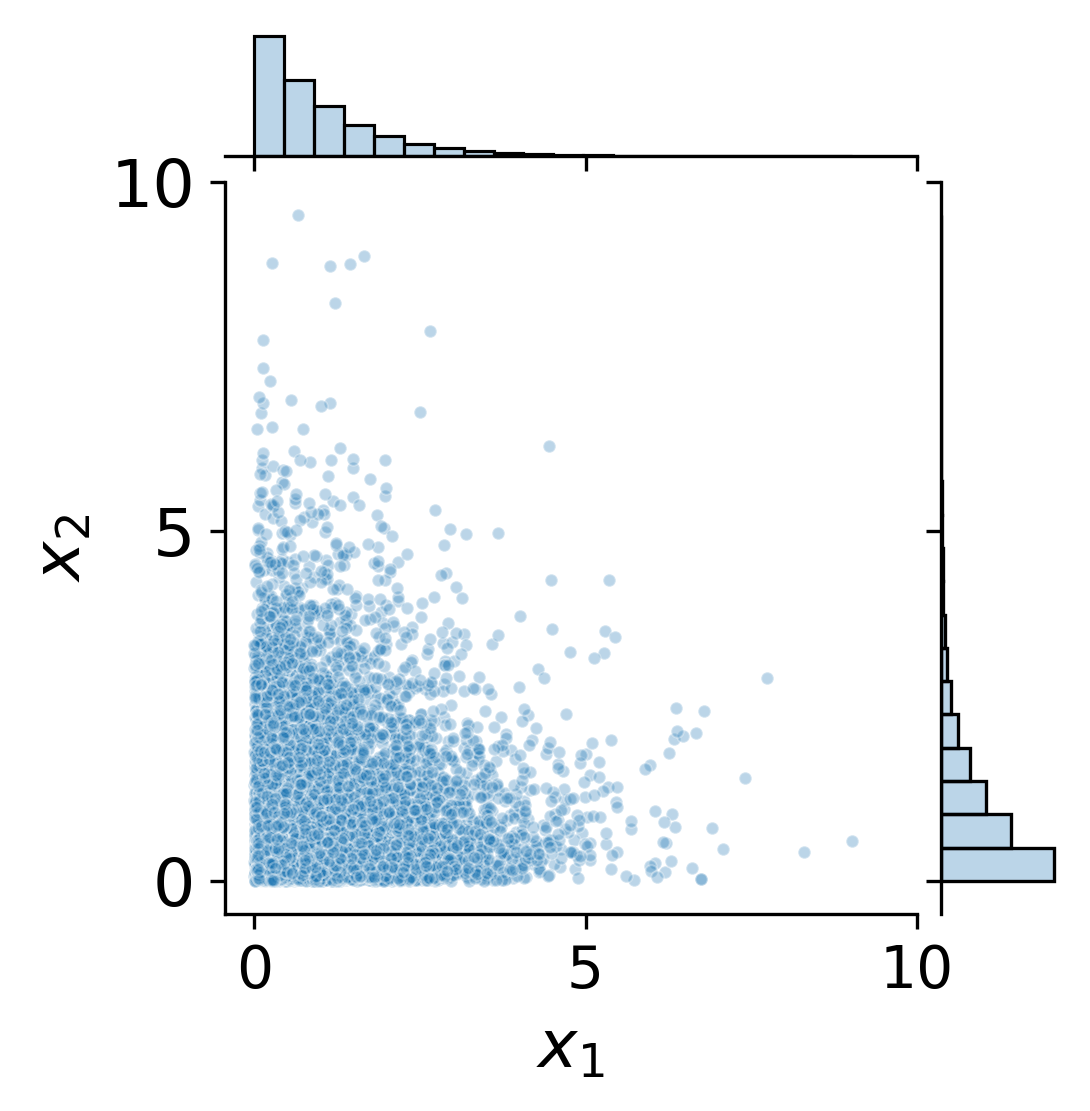
\includegraphics[width=\textwidth]{../numerical_experiments/chapter1/figures/independent_copula.png}
        \caption{Independent copula}
    \end{subfigure}
    \hfill
    \begin{subfigure}[b]{0.32\textwidth}
        \centering
        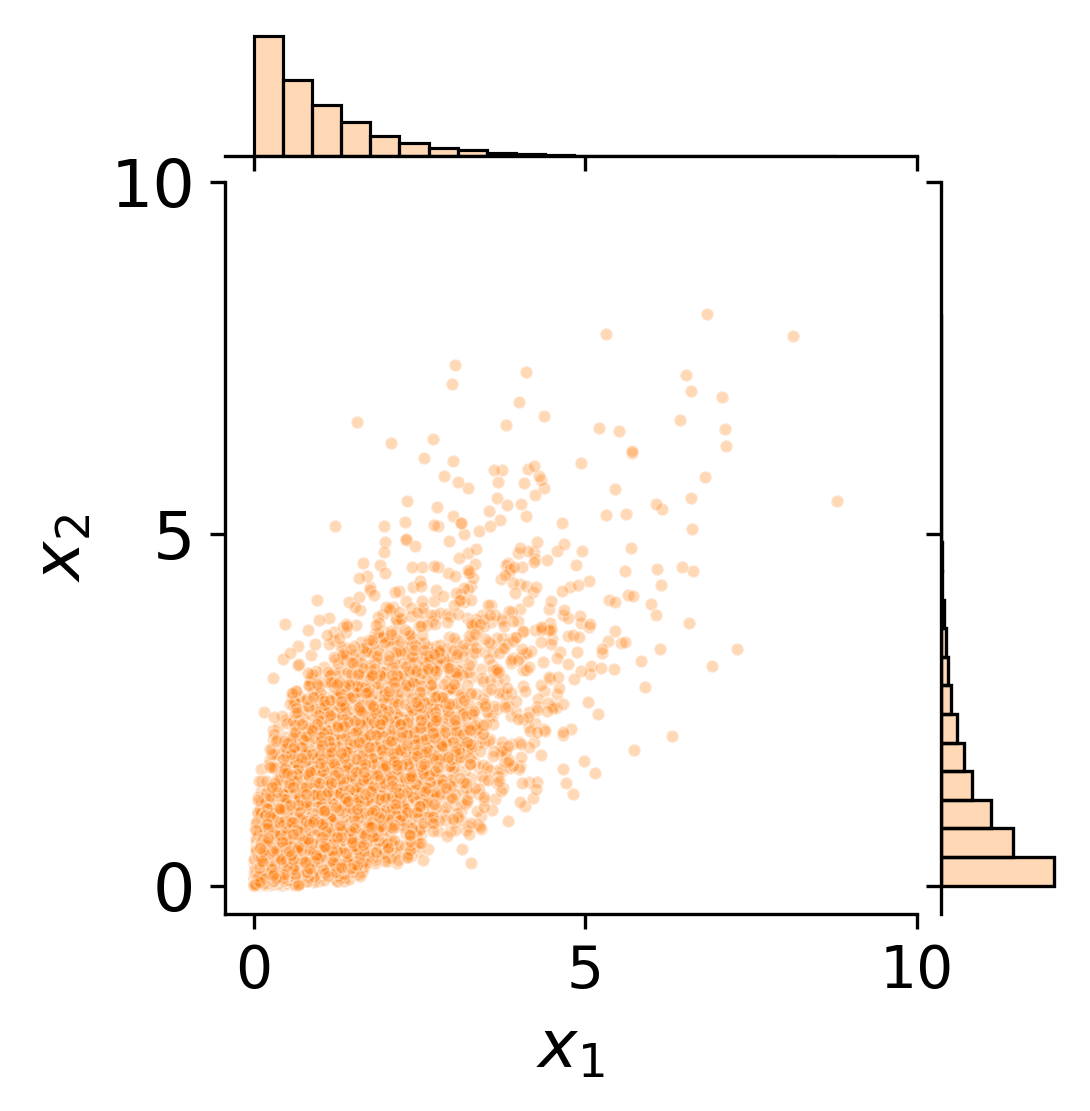
\includegraphics[width=\textwidth]{../numerical_experiments/chapter1/figures/normal_copula.png}
        \caption{Normal copula}
    \end{subfigure}
    \hfill
    \begin{subfigure}[b]{0.32\textwidth}
        \centering
        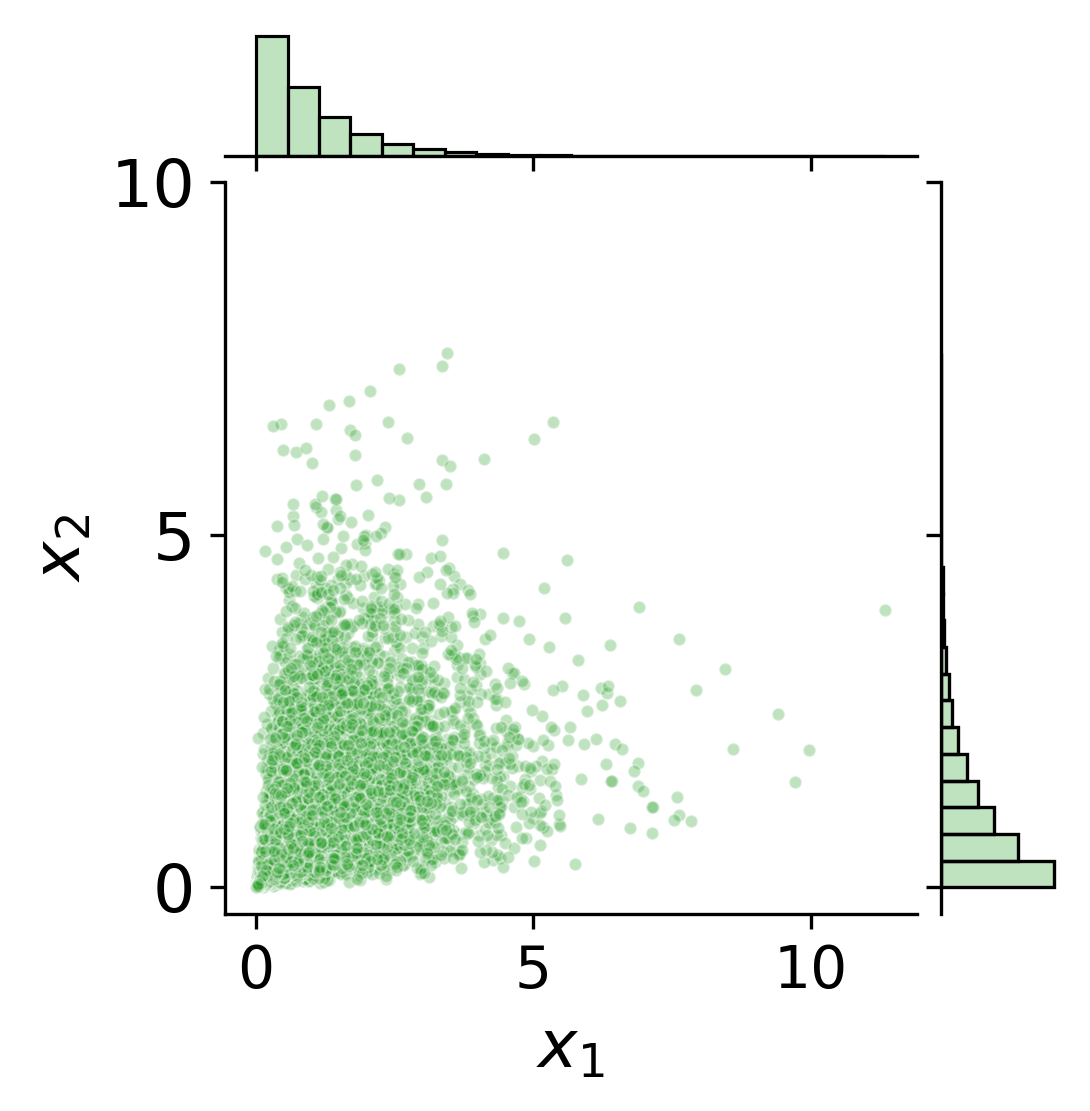
\includegraphics[width=\textwidth]{../numerical_experiments/chapter1/figures/clayton_copula.png}
        \caption{Clayton copula}
    \end{subfigure}
       \caption{Samples of three joint distributions with identical marginals and different dependence structures}
       \label{fig:joint_dist_samples}
\end{figure}

An empirical way of isolating the three dependence structures from this example is to transform the samples in the ranked space. 
Let us consider a $n$-sized sample $\bX_n = \left\{\bx^{(1)}, \dots, \bx^{(n)}\right\} \in \iD_{\bx}^{n}$. 
The corresponding ranked sample is defined as: $\bR_n = \left\{\br^{(1)}, \dots, \br^{(n)}\right\}$, 
where\footnote{The \textit{indicator function} is defined such that $\1_{\left\{\mathcal{A}\right\}}(x) = 1$ if $x \in \mathcal{A}$ and is equal to 0 otherwise.} 
$r^{(l)}_j = \sum_{i=1}^n \1_{\left\{x^{(i)}_j \leq x^{(l)}_j\right\}},$ $\forall j \in \{1, \dots d\}$.
Ranking a multivariate dataset allows us to isolate the dependence structure witnessed empirically. 
\fig{fig:ranked_joint_dist_samples} shows the same three samples from \fig{fig:joint_dist_samples} in the ranked space.
One can first notice that the marginals are uniform since each rank is uniformly distributed. 
Then, the scatter plot from the distribution with independent copula (left plot) is uniform while the two others present different patterns. 
\begin{figure}[ht]
    \centering
    \begin{subfigure}[b]{0.32\textwidth}
        \centering
        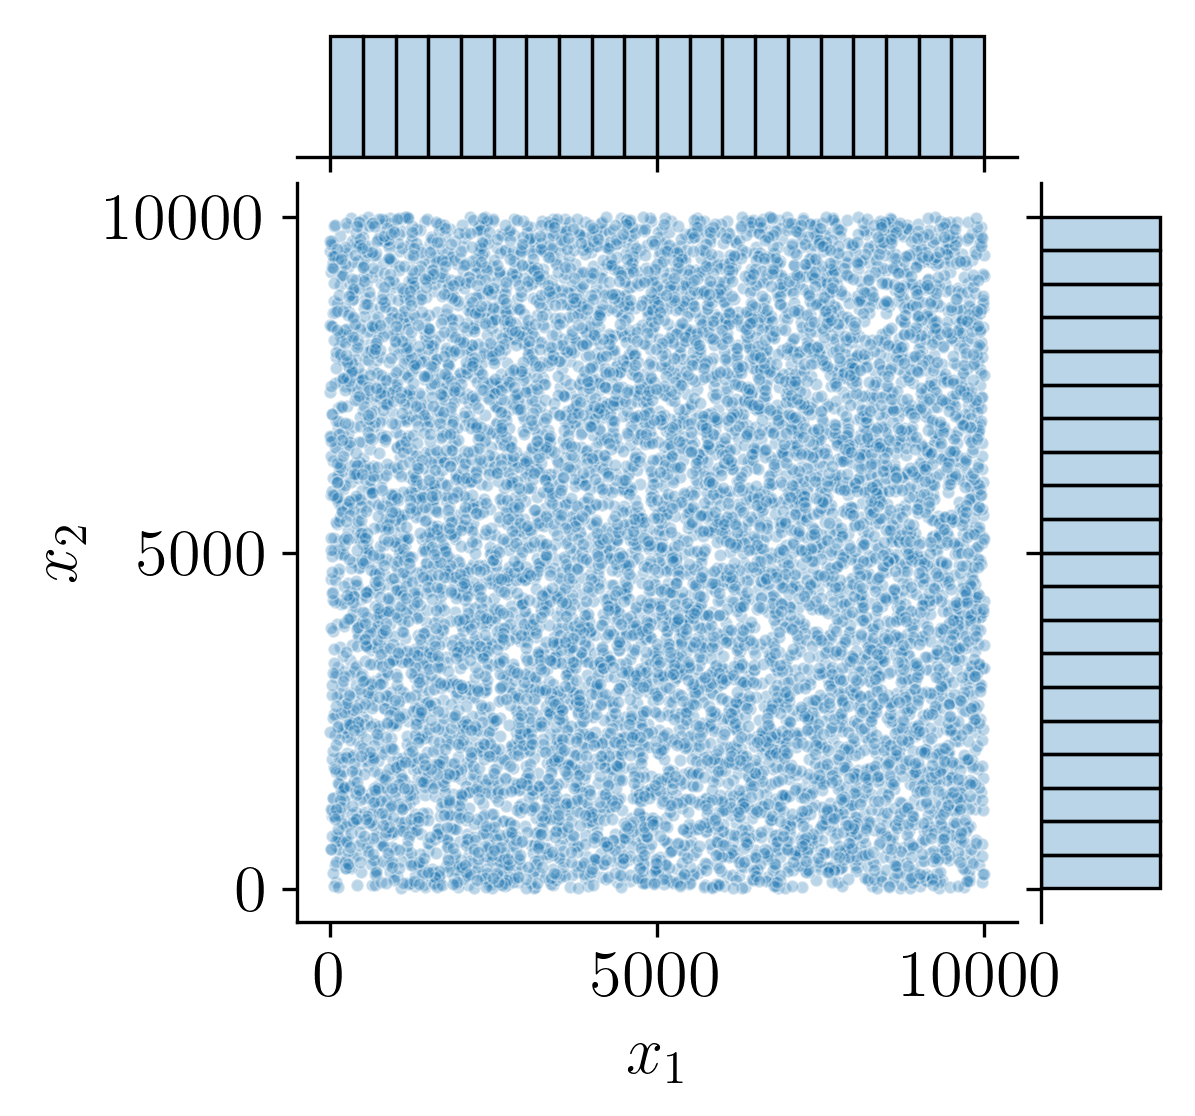
\includegraphics[width=\textwidth]{../numerical_experiments/chapter1/figures/independent_copula_ranked.png}
        \caption{Independent copula}
    \end{subfigure}
    \hfill
    \begin{subfigure}[b]{0.32\textwidth}
        \centering
        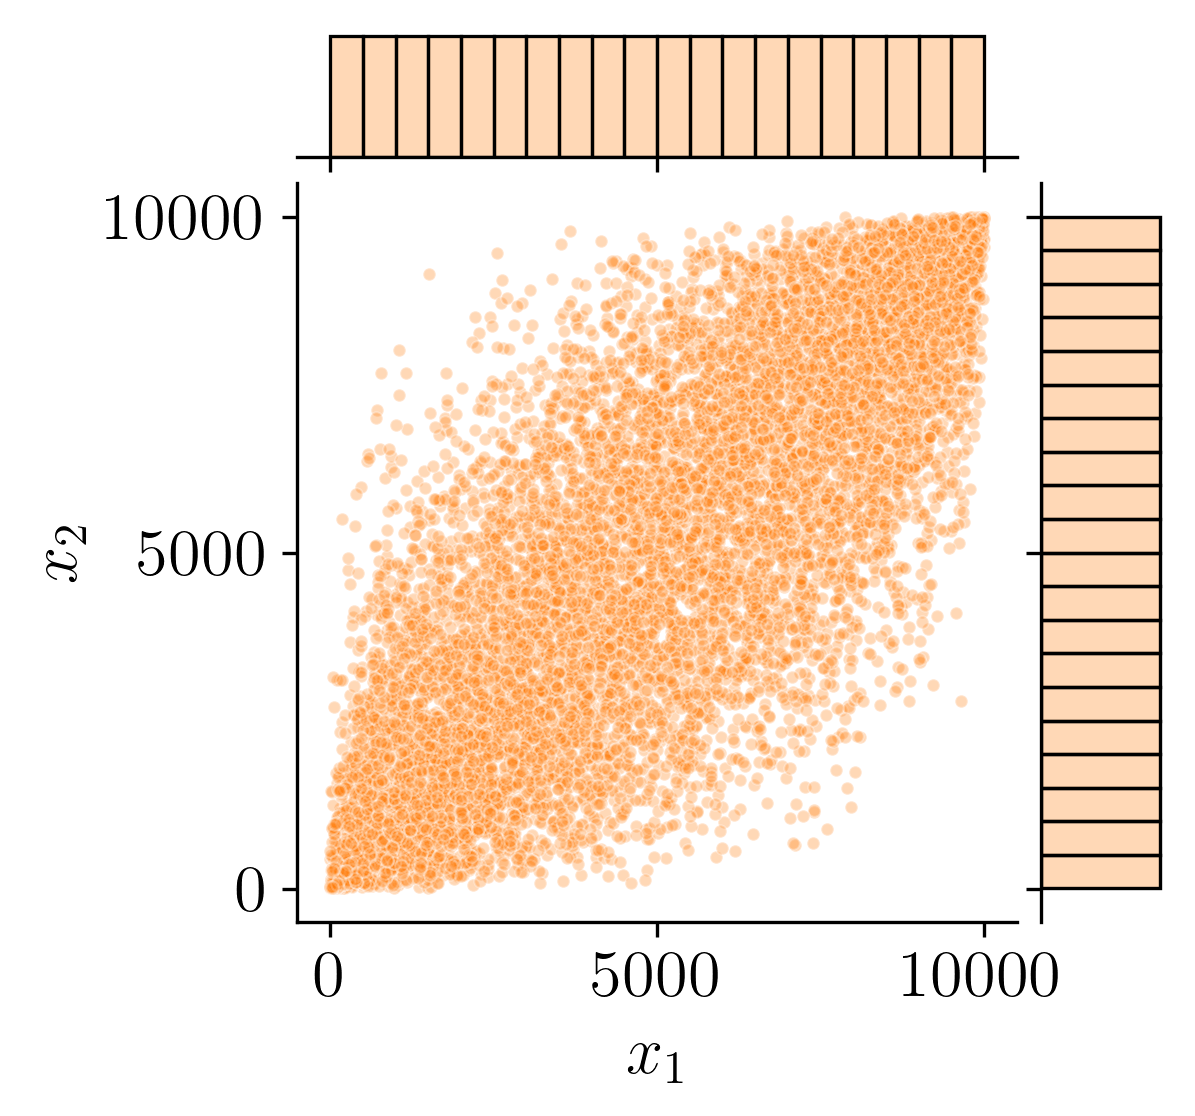
\includegraphics[width=\textwidth]{../numerical_experiments/chapter1/figures/normal_copula_ranked.png}
        \caption{Normal copula}
    \end{subfigure}
    \hfill
    \begin{subfigure}[b]{0.32\textwidth}
        \centering
        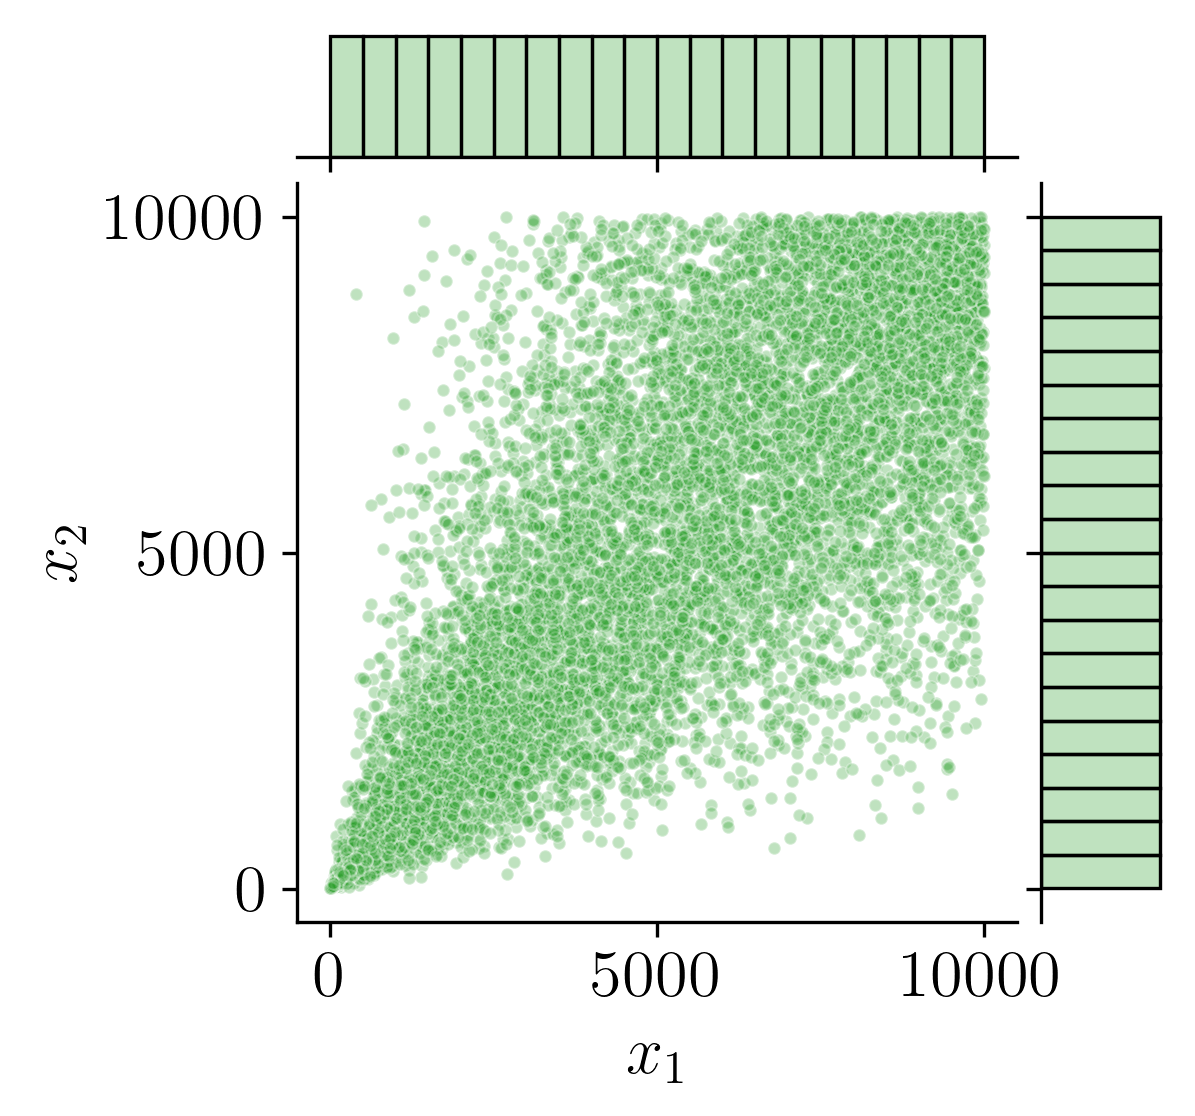
\includegraphics[width=\textwidth]{../numerical_experiments/chapter1/figures/clayton_copula_ranked.png}
        \caption{Clayton copula}
    \end{subfigure}
       \caption{Ranked samples represented in the \fig{fig:joint_dist_samples}}
       \label{fig:ranked_joint_dist_samples}
\end{figure}

A theorem states that the multivariate distribution of any random vector can be broken down into two objects \citep{joe_1997}. 
First, a set of univariate marginal distributions describing the behavior of the individual variables;
Second, a function describing the dependence structure between all variables: a copula. 

\begin{theorem}[Sklar's theorem]
    Let $\mathbf{X} \in \R^d$ be a random vector and its joint CDF $F_{\bX}$ with marginals $\{F_{X_j}\}_{j=1}^d$, there exists a copula $C: [0, 1]^d \rightarrow [0, 1]$, such that:
    \begin{equation}
        F_{\bX}(x_1, \dots, x_d) = C\left(F_{X_1}(x_1), \dots, F_{X_d}(x_d)\right). 
    \end{equation}
    If the marginals $F_{X_i}$ are continuous, then this copula is unique.
    \label{thm:sklar}
\end{theorem}

Theorem \ref{thm:sklar} expresses the joint CDF by combining marginal CDFs and a copula, which is practical for sampling joint distributions. 
Conversely, the copula can be defined by using the joint CDF and the marginal CDFs: 
\begin{equation}
    C(u_1, \dots, u_d) = F_{\bX}(F^{-1}_{X_1}(u_1), \dots, F^{-1}_{X_d}(u_d))
\end{equation}
This equation allows us to extract a copula from a joint distribution by knowing its marginals.
Additionally, copulas are invariant under creasing transformations. 
This property is important to understand the use of rank transformation to display the copula without the marginal effects.     

\elias{define the copula density and address the warning on the confusion.}

Identically to the univariate continuous distributions, a large catalog of families of copulas exists (e.g., independent, Normal, Clayton, Frank, Gumbel copula, etc.).

\elias{define the independent copula, also called a product of marginals.}

To infer a joint distribution, this theorem divides the fitting problem into two independent problems: fitting the marginals and fitting the copula
Provided a dataset, this framework allows the combination of a parametric (or nonparametric) fit of marginals with a parametric (or nonparametric) fit of the copula. 

Appendix \ref{apx:A} details the main techniques to estimate marginal distributions. 
Then, Appendix \ref{apx:B} introduces different nonparametric methods to infer a copula, including the empirical Bernstein copula and the Beta copula. 
The adequation between a fitted probabilistic model and a dataset should be validated, therefore, appendices \ref{apx:A} and \ref{apx:B} respectively present visual and quantitative tools for goodness-if-fit evaluation.

To infer a joint distribution over a dataset, the analyst should determine a fitting strategy.
Smart data visualization helps to choose the fitting methods susceptible to be relevant to the problem. 
The following points can be checked at this early stage: 
\begin{itemize}
    \item Is the distribution unimodal? If not, mixtures methods or nonparametric models might be required;
    \item Is the validity domain restrictive? If so, specific families of parametric distributions can be chosen or truncations can be applied;
    \item Is the dimension high? If the dimension is too high: tensorize the distribution as much as possible.
    \item Is the dependence structure complex? Graphically, the dataset in the ranked space gives an empirical description but some independence tests exist as well. 
\end{itemize} 



%============================================================%
%============================================================%
\section{Central tendency uncertainty propagation}
%============================================================%
%============================================================%

The previous section aimed at building a probabilistic model of the uncertainties considering the knowledge available.
This one will introduce diverse forward propagation of uncertainty through a numerical model. 
This step is hereafter qualified as ``global'' because the analysis of the resulting output random variable will particularly focus on its central tendency (i.e., expected value and variance).
This approach contrasts with the uncertainty propagation dedicated to rare event estimation, which will be introduced in the next section (e.g., for a reliability or certification problem).

The difficulties related to any uncertainty propagation mostly arise from the practical properties of the numerical model. 
Its potential high dimension, low regularity and nonlinearities each represent a challenge. 
These studies rely on a finite number of observations which depends on the computational budget the analyst can afford.   
This forward propagation might be a finality of the uncertainty quantification, but keep in mind that it fully stands on an accurate uncertainty modeling.
Uncertainty propagation should be perceived as a standardized process with modular bricks, on which the ``garbage in, garbage out'' concept fully applies.

This section introduces the main methods of global uncertainty propagation. 
Outlining the strong links between numerical integration (i.e., Lebesgue integration or central tendency estimation) and numerical design of experiments. 


%============================================================%
\subsection{Numerical integration}
%============================================================%

Forward uncertainty propagation aims at integrating a measurable function $g: \iD_{\bX} \rightarrow \R$ with respect to a probability measure $\mu$.
Numerical integration brings algorithmic tools to help the resolution of this probabilistic integration (i.e., Lebesgue integration). 

In practice, this integral is approximated by summing a finite $n$-sized set of realizations $\by_n = \left\{g(\bx^{(1)}), \dots, g(\bx^{(n)})\right\}$ from a set of input samples $\bX_n = \left\{\bx^{(1)}, \dots, \bx^{(n)}\right\}$. 
A \textit{quadrature} establishes a rule to select the input samples $\bX_n$ (also called nodes), and an associated set of weights $\bw_n = \{w_1, \dots, w_n\} \in \R^n$. 
The approximation given by a quadrature rule is defined as a weighted arithmetic mean of the realizations:
\begin{equation}
    I_{\mu}(g) := \int_{\iD_\bX} g(\bx) \dd\mu(\bx) \approx \sum_{i=1}^n w_i g\left(\bx^{(i)}\right).
    \label{eq:quadrature_rule}
\end{equation}
For a given sample size $n$, our goal is to find a set of tuples $\left\{\bx^{(i)}, w_i \right\}_{i=1}^n$ (i.e., quadrature rule), giving the best approximation of our quantity. 
Ideally, the approximation quality should be fulfilled for a wide class of integrands. 
Most quadrature rules only depend on the measure space $(\Omega, \iA, \mu)$, regardless of the integrand values.
In the context of a costly numerical model, this property allows the analyst to massively distribute the calls to the numerical model. 

This section aims at presenting the main multivariate numerical integration techniques. 
These methods have very different properties: 
some are deterministic and some are aleatory; 
some are sequential (or nested) some are not; 
some are victims of the curse of dimensionality and some are not. 
\elias{A summary table of the different methods and their respective properties is proposed ADD REF TO TABLE}.

%\item Some quadratures define negative weights, which can introduce numerical instabilities when $n$ gets large.
%\item The nature of the probability measure (i.e., presence of dependence) might restrict the use of methods

%------------------------------------------------------------%
\subsubsection{Classical multivariate deterministic quadrature}
%------------------------------------------------------------%

Historically, quadrature methods have been developed for univariate integrals. 
The Gaussian rule and the Fejér-Clenshaw-Curtis rule are two univariate deterministic quadratures that will be briefly introduced. 

%Let us first mention the Newton-Cotes quadratures, generalizing multiple rules (e.g., the trapezoidal rule, Simpson's rule, etc.).
Gaussian quadrature is a powerful univariate quadrature building together a set of irregular nodes and a set of weights. 
The computed weights are positive, which ensures a numerically stable rule even for large sample sizes.

Different variants of rules exist, the most famous being the Gauss-Legendre quadrature. 
In this case, the function $g$ to be integrated with respect to the uniform measure on $[-1, 1]$ is approximated by Legendre polynomials.
Considering the Legendre polynomial of order $n$, denoted $l_n$, the quadrature nodes ${x^{(i)}}_{i=1}^n$ are given by the polymonial roots.
The respective weights are given by the following formula: 
\begin{equation}
    w_{i}={\frac {2}{\left(1-\left(x^{(i)}\right)^{2}\right)\left(l'_{n}(x^{(i)})\right)^{2}}}.
\end{equation}
This rule guarantees a very precise approximation provided that the integrand is well-approximated by a polynomial of degree $2n-1$ or less on $[-1, 1]$.
This rule is deterministic but not sequential, meaning that two rules with sizes $n_1$ and $n_2$, $n_1 < n_2$ will not be nested. 
However, a sequential extension is proposed by the Gauss-Kronrod rule \citep{laurie_1997}, offering lower accuracy. 

To overcome this practical drawback, Fejér then Clenshaw with Curtis proposed a nested rule with mostly equivalent accuracy as Gaussian quadrature.
This method is usually presented to integrate a function with respect to the uniform measure on $[-1, 1]$ and starts with a change of variables:
\begin{equation}
    \int_{-1}^{1} g(x) \, \dd x = \int_{0}^{\pi} g(\cos(\theta)) \sin(\theta) \, \dd \theta 
\end{equation}
This expression can be written as an expansion of the integrand using cosine series. 
Moreover, cosine series are closely related to the Chebyshev polynomials of the first kind. 
Fejér's ``first rule'' \citep{trefethen_2008} relies on the Chebyshev polynomials roots as nodes $x^{(i)} = \cos(\theta^{(i+1/2)})$, and the following weights:
\begin{equation}
    w_i=\frac{2}{n}\left(1-2\sum_{j=1}^{\lfloor n/2 \rfloor}\frac{1}{4j^2-1}\cos\left(j\theta^{(2i+1)}\right)\right)    
\end{equation}
These two univariate integration schemes are both very efficient on a wide panel of functions. 
Yet, Fejér-Clenshaw-Curtis is sequential and offers easy implementations, benefitting from powerful algorithms such as the \textit{fast Fourier transform}. 

\begin{figure}[ht]
    \centering
    \begin{subfigure}[b]{0.32\textwidth}
        \centering
        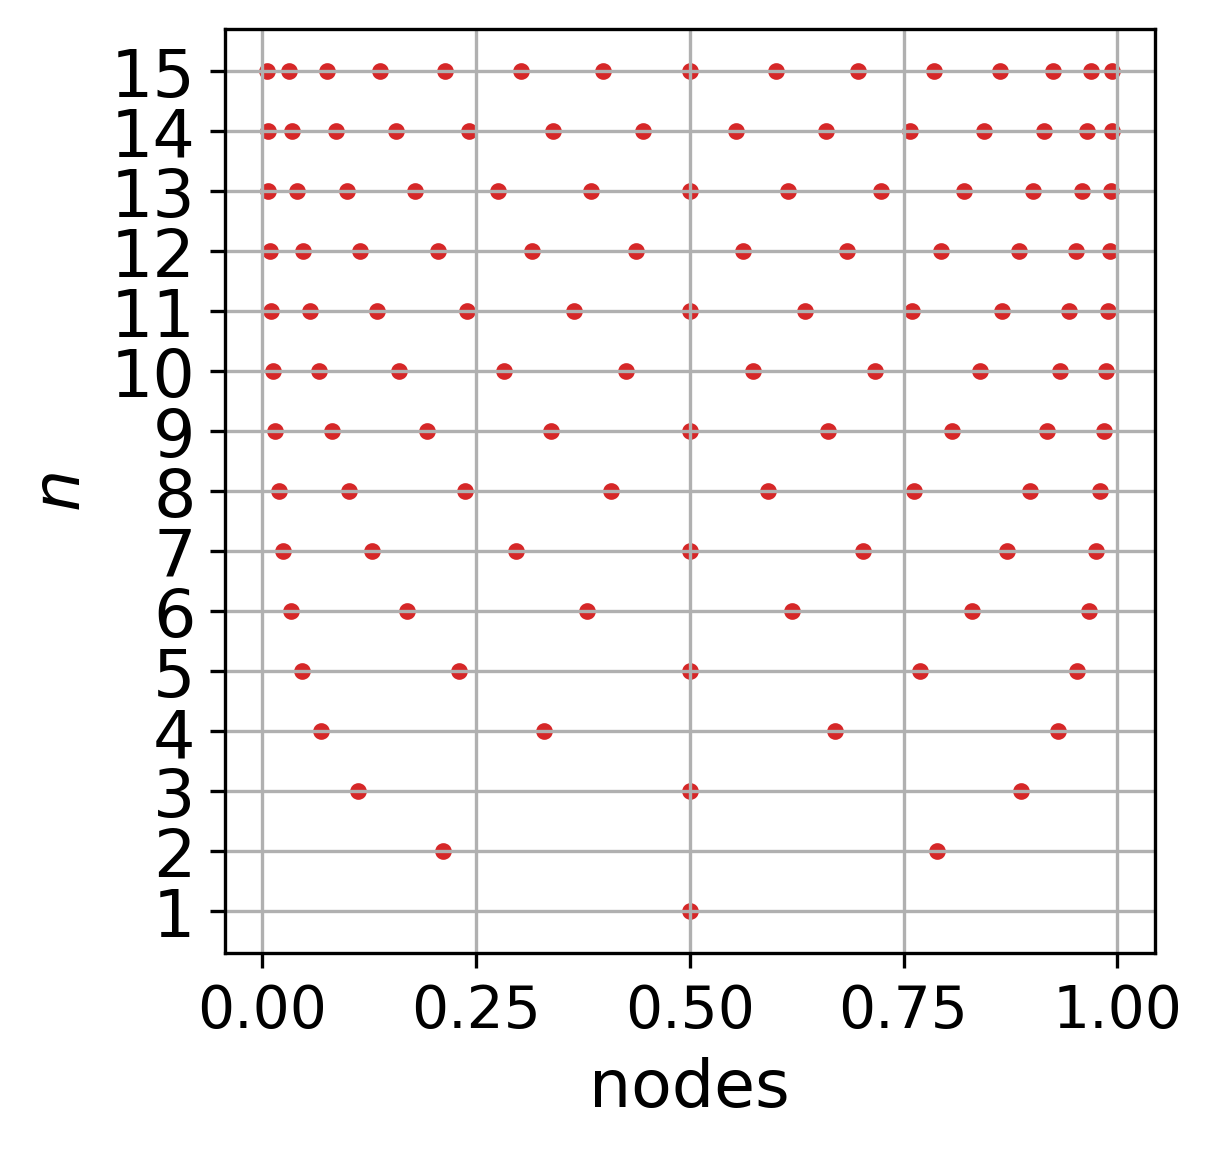
\includegraphics[width=\textwidth]{../numerical_experiments/chapter1/figures/univariate_gauss_legendre.png}
        \caption{Gauss-Legendre}
    \end{subfigure}
    \quad
    \begin{subfigure}[b]{0.32\textwidth}
        \centering
        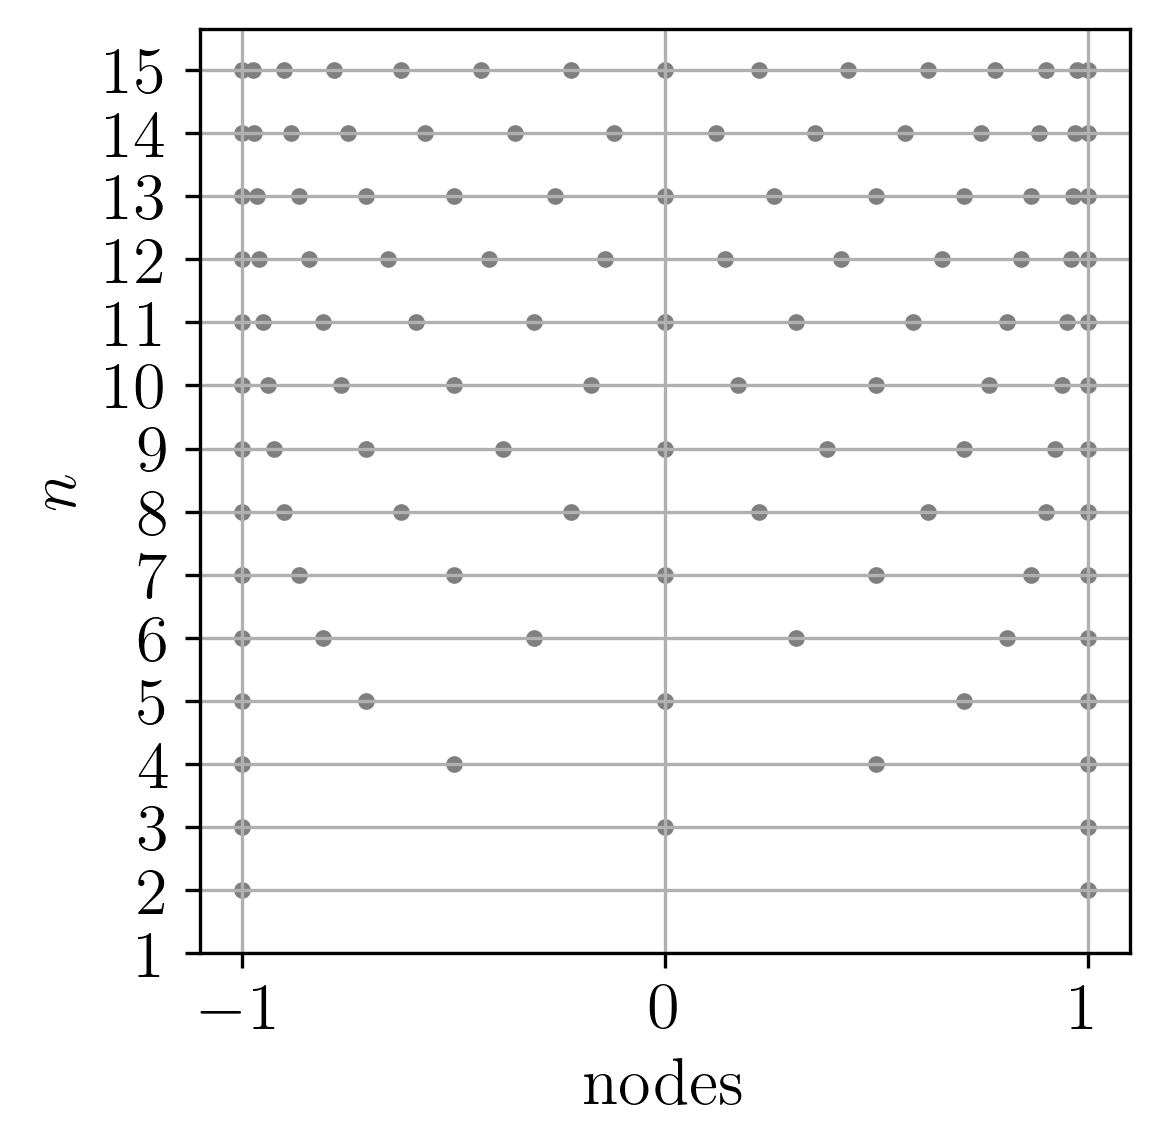
\includegraphics[width=\textwidth]{../numerical_experiments/chapter1/figures/univariate_clenshaw_curtis.png}
        \caption{Clenshaw-Curtis}
    \end{subfigure}
    \caption{Univariate quadratures nodes ($1 \leq n \leq 15$)}
    \label{fig:univariate_quads}
\end{figure}


Uncertainty quantification problems are rarely unidimensional, but one can build a multivariate quadrature rule by defining the tensor product (also called full grids) of univariate rules. 
This exhaustive approach quickly shows its practical limits as the problem's dimension increases. 
Alternatively, sparse multivariate quadratures (i.e., Smolyak sparse grid) explore the joint domain more efficiently. 



%------------------------------------------------------------%
\subsubsection{Monte Carlo methods}
%------------------------------------------------------------%
Monte Carlo methods were initially developed in the 1940s to solve problems in neutronics.  
Ever since this frequentist techniques have been applied to the resolution of the Lebesgue integral. 
To integrate a function $g$ against a measure $\mu$, it randomly generates points following the input measure. 
The integral is estimated by taking the uniform arithmetic mean of the images of these nodes obtained by this random process. 

This aleatory method requires to be able to generate points following a given distribution. 
To do so, the most common approach is to first generate a sequence of random points uniformly on $[0, 1]$. 
These sequences mimic actual uniform randomness but are in fact generated by deterministic algorithms (also called pseudorandom number generators).
Pseudorandom algorithms generate a sequence of numbers with a very large, but finite length. 
This sequence can be exactly repeated by fixing the same initial point, also called \textit{pseudorandom seed}.
Most programming languages use the Mersenne Twister pseudorandom generator \citep{matsumoto_1998}, offering a very long period (around $4.3\times10^{6001}$ iterations).

Formally, the ``Vanilla'' Monte Carlo (sometimes called ``crude'' Monte Carlo) method uses a set of i.i.d samples $\bX_n = \left\{\bx^{(1)}, \dots, \bx^{(n)}\right\}$ following the joint distribution of $\mu$. 
The Monte Carlo estimator of the integral is given by: 
\begin{equation}
    I_{\mu}(g) \approx \Bar{y}_n^{\textrm{MC}} = \frac1n \sum_{i=1}^{n} g(\bx^{(i)}).
\end{equation}
By construction, the law of large numbers makes this estimator unbiased, however, it converges relatively slowly. 
Considering the images of the sample $\bX_n$, one can also estimate the variance of the output random variable $\what{\sigma}^2_Y$.
The variance of the Monte Carlo estimator results from a manipulation of the central tendency theorem:
\begin{equation}
    \var\left(\Bar{y}_n^{\textrm{MC}}\right) = \frac{1}{\sqrt{n}} \var\left(g(\bX)\right). 
\end{equation}
This estimator also comes with theoretical confidence intervals at $\alpha \%$, regardless of the output distribution: 
\begin{equation}
    I_{\mu}(g) \in \left[\Bar{y}_n^{\textrm{MC}}  - q_\alpha \frac{\var\left(g(\bX)\right)}{\sqrt{n}}, \Bar{y}_n^{\textrm{MC}}  + q_\alpha \frac{\var\left(g(\bX)\right)}{\sqrt{n}} \right],
\end{equation}
where $q_\alpha$ is the $\alpha$-quantile of the standard normal distribution.
Monte Carlo presents the advantage of being a universal method, with no bias and strong convergence guarantees. 
Moreover, it is worth noting that its convergence properties do not depend on the dimension of the input domain. 
Unlike the previous multivariate deterministic quadrature, Monte Carlo doesn't suffer from the curse of dimensionality. 
The main limit of crude Monte Carlo is its convergence speed, making it untractable in most practical cases. 
More recent methods aim at keeping the interesting properties of this technique while making it more efficient.
Among the \textit{variance reduction} family of methods, let us mention importance sampling, stratified sampling (e.g., latin hypercube sampling), control variates and multi-level Monte Carlo (see Chapters 8, 9 and 10 from \citet{owen_2013} and \citep{giles_2008}).


%------------------------------------------------------------%
\subsubsection{Quasi-Monte Carlo and Koksma-Hlawka inequality}
%------------------------------------------------------------%

Among the methods presented so far, classical deterministic quadratures are subject to the curse of dim while Monte Carlo methods deliver contrasted performances. 
Quasi-Monte Carlo is a deterministic family of numerical integration schemes over $[0, 1]^d$ with respect to the uniform measure on $[0, 1]$. 
It offers powerful performances with strong guarantees by choosing nodes respecting \textit{low discrepancy} sequences. 

The discrepancy of a set of nodes (or a design) can be seen as a metric of its uniformity. 
The lowest the discrepancy of a design is, the ``closest'' it is to uniformity. 

The Koksma-Hlawka theorem \citep*{morokoff_1995,leobacher_2014} is a fundamental result for understanding the role of the discrepancy in numerical integration. 
\begin{theorem}[Koksma-Hlawka]
    If $g:[0, 1]^d\rightarrow\R$ has a bounded variation (i.e., its total variation is finite), then for any design $\bX_n = \left\{\bx^{(1)}, \dots, \bx^{(n)}\right\} \in [0, 1]^d$:
    \begin{equation}
        \left| \int_{[0, 1]^d} g(\bx) \ddx - \frac1n \sum_{i=1}^n g\left(\bx^{(i)}\right)\right| \leq  V(g) D^*(\bX_n).
        \label{eq:KH_inequality}
    \end{equation}

    Where $D^*(\bX_n)$ is the star discrepancy of the design $\bX_n$, while $V(g)$ quantifies the complexity of the integrand, which is related to its total variation. 
\end{theorem}

Where the function variation $V(g)$ in the \eq{eq:KH_inequality} can formally be defined as the Hardy-Klause variation: 
\begin{equation}
    V(g) = \sum_{\mathfrak{u}\subseteq\{1, \dots, p \}} \int_{[0, 1]^\mathfrak{u}} \left| \frac{\partial^{\mathfrak{u}}g}{\partial \bx_{\mathfrak{u}}}(\bx_{\mathfrak{u}}, 1)\right| \dd\bx.
\end{equation}

Where the \textit{$L_p$ star discrepancy} of a design $\bX_n$ defined as the $L_p$-norm of the difference between the empirical CDF of the design $\what{F}_{\bX_n}$ and the CDF of the uniform distribution $F_{\textbf{U}}$:  
\begin{equation}
    D^*_p(\bX_n) = \lVert \what{F}_{\bX_n} - F_{\textbf{U}}\rVert _p = \left(\int_{[0, 1]^d} \lvert\what{F}_{\bX_n}(\bx) - F_{\textbf{U}}(\bx)\rvert ^p \, \ddx \right)^{1/p}.
\end{equation}
Additionally, the $L_\infty$ star discrepancy can be defined from a geometric point of view. 
Let us consider the number of a design $\bX_n$, falling in a subdomain $[\mathbf{0}, \bx)$ as $\#(\bX_n \cap [\mathbf{0}, \bx))$. 
Then, this empirical quantification is compared with the volume of the rectangle $[\mathbf{0}, \bx)$, noted $\mathrm{vol}\left([\mathbf{0}, \bx)\right)$.  
Finally, this star discrepancy is written:   
\begin{equation}
    D^*(\bX_n) = \sup_{\bx \in [0, 1]^d} \left| \frac{\#(\bX_n \cap [\mathbf{0}, \bx))}{n} - \mathrm{vol}\left([\mathbf{0}, \bx)\right)\right|
\end{equation}
\elias{Figure xx empirically represents discrepancy concept}
Let us point out that this star discrepancy is equivalent to the Kolmogorov-Smirnov test verifying whether the design follows a uniform distribution. 

\noindent
One can notice how the Koksma-Hlawka inequality dissociates the quadrature performance into a contribution from the function complexity and one from the repartition of the quadrature nodes. 
Knowing that the complexity of the studied integrand is fixed, this property explains the motivation to generate low-discrepancy quadratures in numerical integration.  

Note that the design can also be considered as a discrete distribution (uniform sum of Dirac distributions).
The discrepancy can then be expressed as a probabilistic distance between this discrete distribution and the uniform distribution. 
A generalized discrepancy between distributions will be presented in the \elias{Part 2}.

Some famous low-discrepancy sequences (e.g., van der Corput, Halton, Sobol', Faure, etc.) can offer a bounded star discrepancy $D^*(\bX_n) \leq \frac{C \log(n)^d}{n}$, with $C$ a constant depending on the sequence.
Therefore, using these sequences as a quadrature rule with uniform weights provides the following absolute error upper bound: 
\begin{equation}
    \left| \int_{[0, 1]^d} g(\bx) \ddx - \frac1n \sum_{i=1}^n g\left(\bx^{(i)}\right)\right| \leq  \frac{V(g) \log(n)^d}{n}
\end{equation}

%This bound is qualified as sharp since for any design $\bX_n$, and every $\epsilon > 0$, a function $g$ with variation $V(g)=1$ exists such that:
%\begin{equation}
%    \left| \int_{[0, 1]^d} g(\bx) \ddx - \frac1n \sum_{i=1}^n g\left(\bx^{(i)}\right)\right|  > D^*(\bX_n) - \epsilon.
%\end{equation} 

The generation of these sequences doesn't necessarily require more effort than pseudo-random sampling.
Chapter 15 in \citet{owen_2013} offers an extended presentation of the ways to generate different low-discrepancy sequences. 
For example, the van der Corput and Halton sequences rely on congruential generators. 
%Then, scrambling procedures are sometimes implemented to correct pathologies famously observed on Halton sequences. 
To overcome the limits of Halton sequences, digital nets such as the famous Sobol' or Faure sequences have been developed.  
Sobol' sequences are in base two and have the advantage of being extensible in dimension. 
Note that by construction, these sequences offer significantly lower discrepancies for specific values. 
Typically designs with sizes equal to powers of two or power of prime numbers will be favorable. 
To illustrate the different patterns and properties of different methods, \fig{fig:quasi_monte_carlo_designs} represents the three designs of 256 points. 
Each is split into the first 128 points (in red) and the following 128 points (in black) to show to nested properties of the QMC sequences.

\begin{figure}[ht]
    \centering
    \begin{subfigure}[b]{0.32\textwidth}
        \centering
        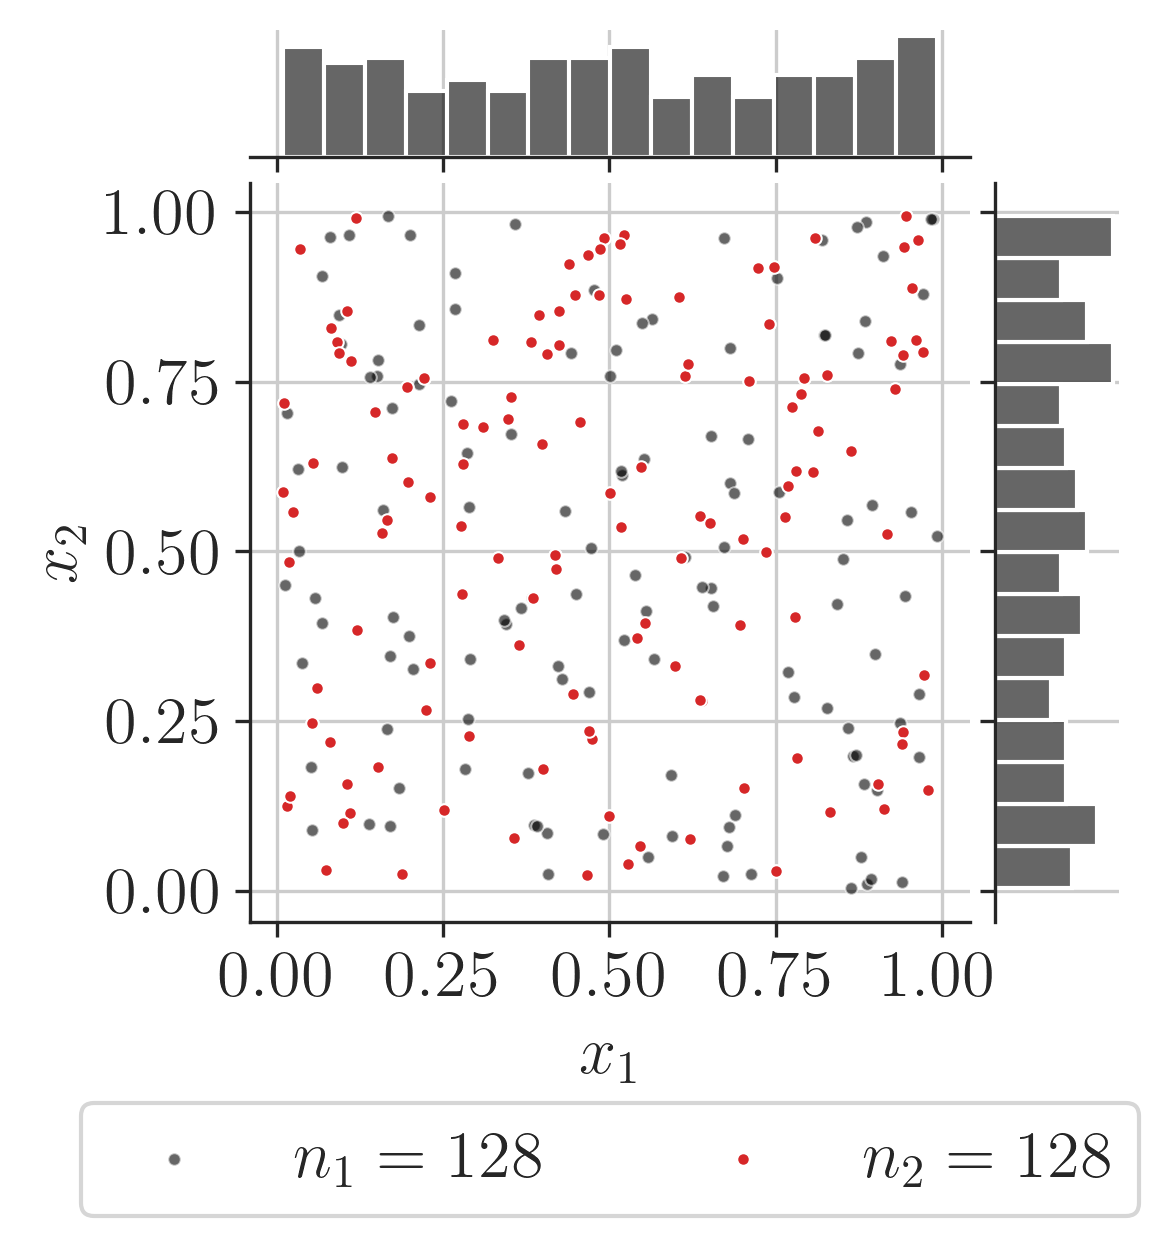
\includegraphics[width=\textwidth]{../numerical_experiments/chapter1/figures/MonteCarlo256.png}
        \caption{Monte Carlo}
    \end{subfigure}
    \hfill
    \begin{subfigure}[b]{0.32\textwidth}
        \centering
        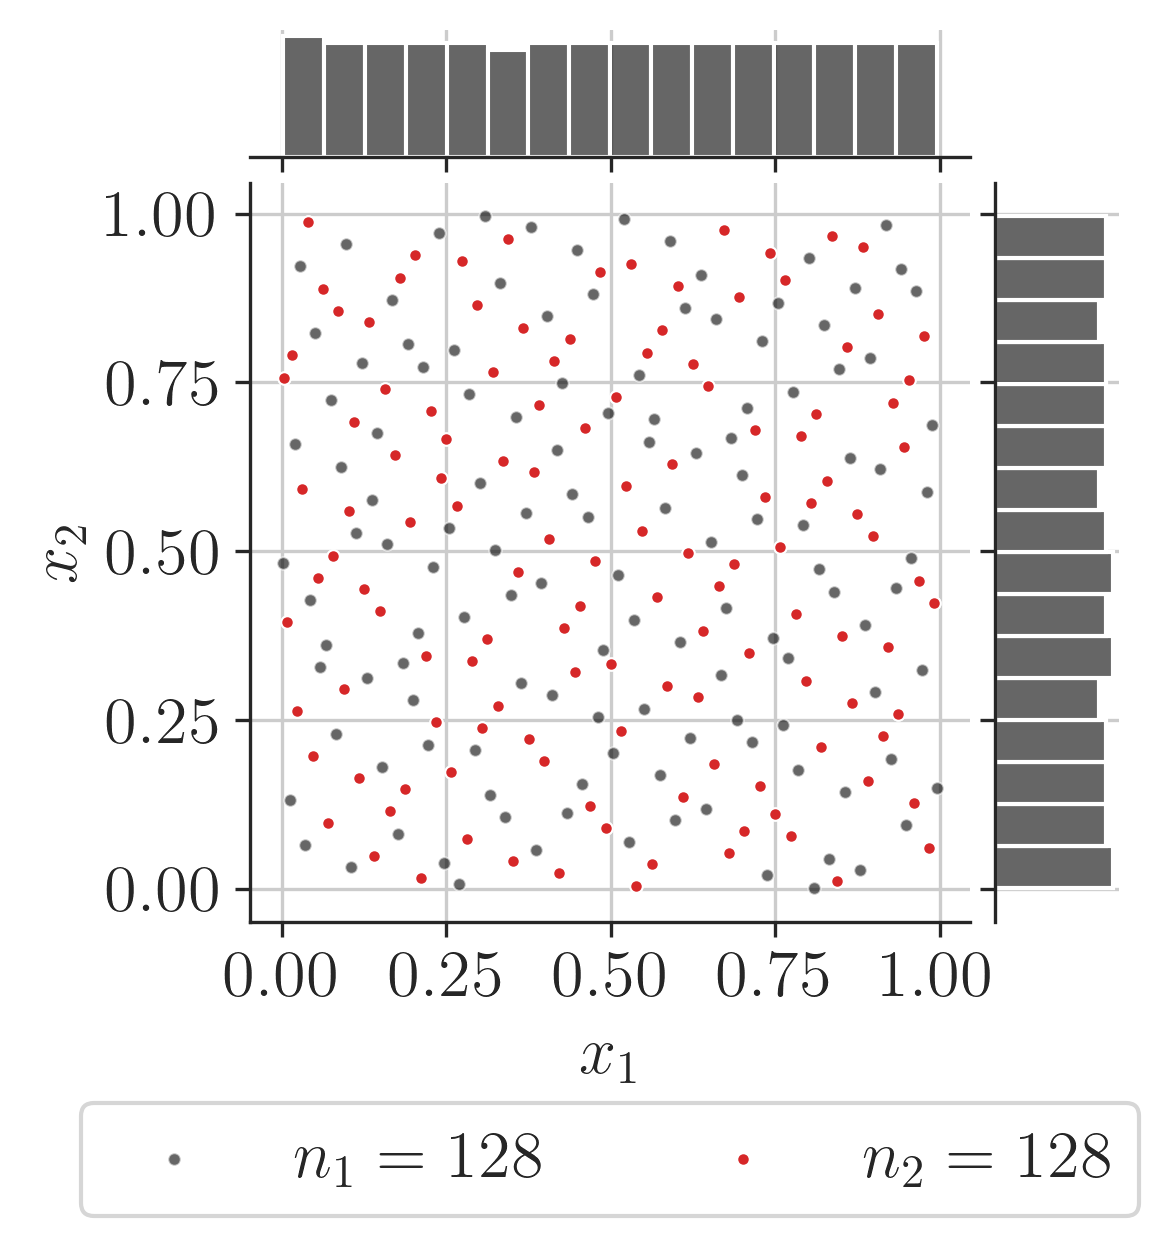
\includegraphics[width=\textwidth]{../numerical_experiments/chapter1/figures/quasi_MonteCarlo_Halton_256.png}
        \caption{Halton sequence}
    \end{subfigure}
    \hfill
    \begin{subfigure}[b]{0.32\textwidth}
        \centering
        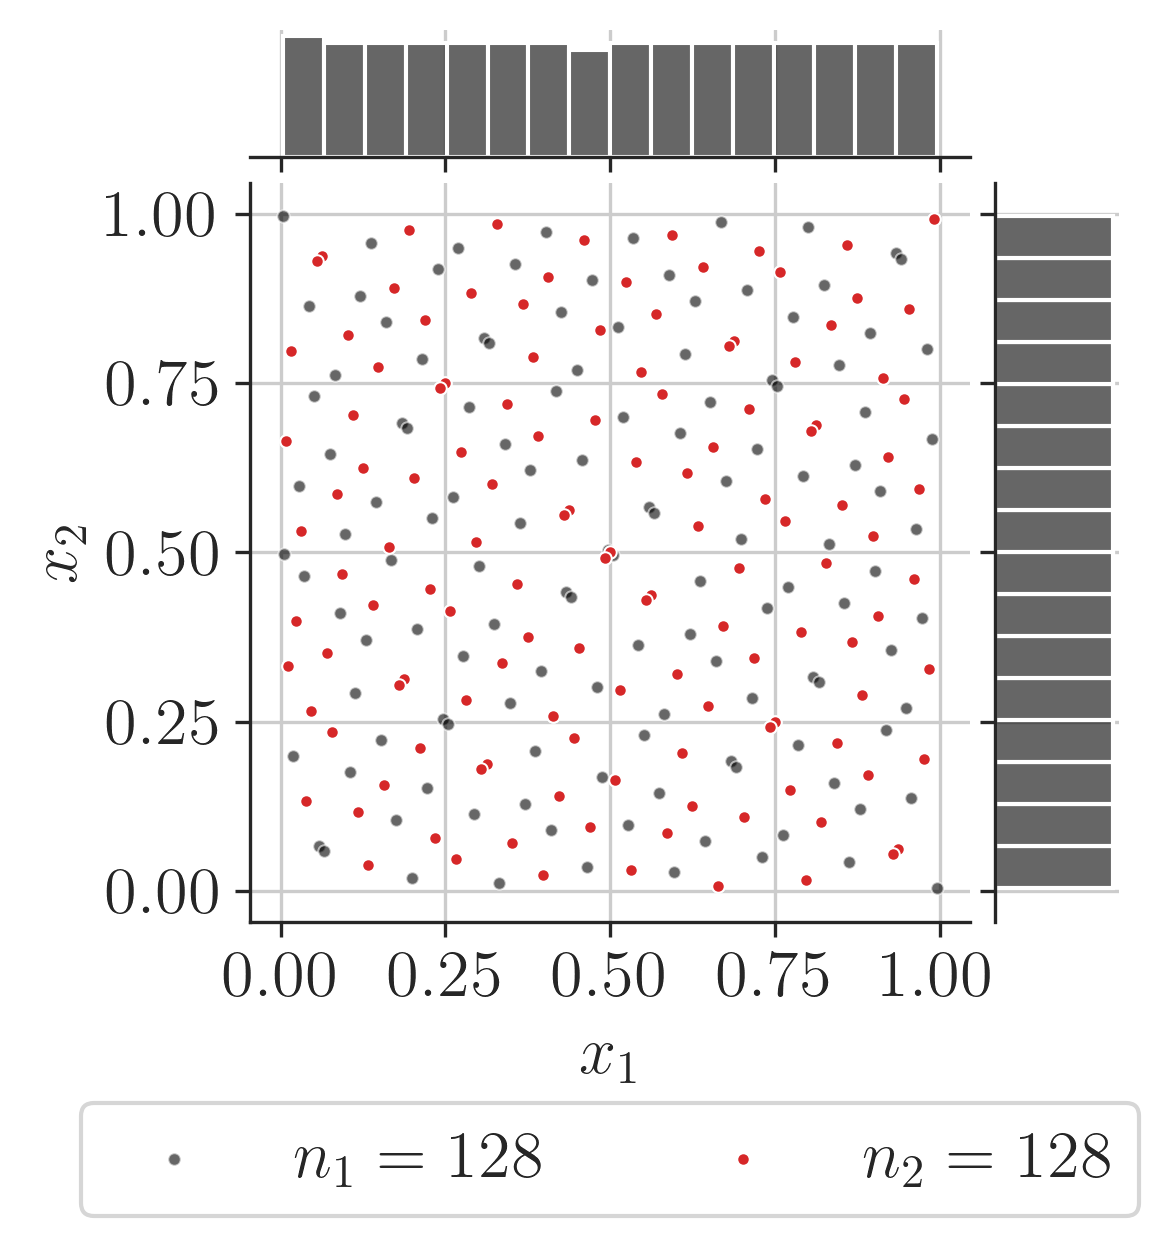
\includegraphics[width=\textwidth]{../numerical_experiments/chapter1/figures/quasi_MonteCarlo_256.png}
        \caption{Sobol' sequence}
    \end{subfigure}
       \caption{Nested Monte Carlo and quasi-Monte Carlo designs ($n=256$)}
       \label{fig:quasi_monte_carlo_designs}
\end{figure}

A quantity estimated by crude MC comes with some associated confidence. 
This complementary information is essential to deliver an end-to-end uncertainty quantification and misses in QMC methods.  
\textit{Randomized quasi-Monte Carlo} (RQMC) is a method adding some randomness in QMC in order to compute confidence intervals while benefiting from a low variance.
A specific review of the randomized (also called ``scrambled'') QMC is proposed by \citet{lecuyer_2018}. Various authors recommend the use of RQMC by default instead of QMC as a good practice. 
Recent works aim at exploring the use of these methods to estimate different quantities of interest (such as an expected value \citep{gobet_2022} or a quantile \citep{tuffin_2019})

Quasi-Monte Carlo methods easily generate powerful integration schemes. 
The KH inequality associates an upper bound and a convergence rate to most integrals. 
A randomization overlay fades the deterministic property of these designs to allow confidence interval computation.
In the following, sampling techniques are presented from the numerical \textit{design of experiments} point of view. 
Even if the finality might look different from the previous numerical integration, it shares many methods and concepts. 



%============================================================%
\subsection{Numerical design of experiments}
%============================================================%
The numerical design of experiments aims at exploring uniformly the input domain, e.g., to build the learning set of a regression model, or to initialize a multi-start optimization strategy. 
A design of experience (also simply called design) is then qualified as \textit{space-filling} when it properly covers a domain. 
As well as in integration, a design of experiments allows propagating uncertainties through a numerical model (or an actual experiment from a laboratory test bench). 
However, a difference comes from the fact that this community often works with designs of very limited sizes. 
Users of designs of experiments might also need to build designs with various properties. 
\begin{itemize}
    \item Some might be interested in the sequentiality of a sampling method, to eventually add new points as they get a computational budget extension.
    \item Some might request a sampling method conserving its properties in any sub-domains. 
    This second property can be useful to reduce the problem's dimension by dropping a few unimportant marginals.
\end{itemize}

Different metrics are commonly used to quantify how space-filling a design of experiments is. 
The previously introduced different types of discrepancies are space-filling metrics.
Other types of space-filling metrics rely on purely geometrical considerations.  

This section will first define some space-filling metrics.
Secondly, the \textit{latin hypercube sampling} (LHS) will be introduced as a variance-reduction that became popular in this community. 
Finally, a general discussion on uncertainty propagation with respect to non-uniform measures will be presented.

%------------------------------------------------------------%
\subsubsection{Space-filling metrics and properties}
%------------------------------------------------------------%
Space-filling criteria are key to evaluating designs and are often used in their construction to optimize their performances. 
In the previous section, the star discrepancy was introduced as a distance of a finite design to uniformity.
However, the $L_\infty$ star discrepancy is hard to estimate, fortunately, \citet{warnock_1972} elaborated an explicit expression specific to the $L_2$ star discrepancy: 
\begin{equation}
    \left[D^*_2(\bX_n)\right]^2 = \frac19 - \frac2n \sum_{i=1}^{n} \prod_{l=1}^{d} \frac{(1-x_l^{(i)})}{2} + \frac{1}{n^2}\sum_{i,j=1}^{n} \prod_{l=1}^{d} \left[1 - \max(x_l^{(i)}, x_l^{(j)})\right].
\end{equation}
One can notice that this expression is similar to the Cramér-von Mises test statistic. 
Even if this expression is tractable, \citet{fang_liu_2018} detailed its limits. 
First, the star $L_2$ discrepancy generates designs that are not robust to projections in sub-spaces. 
Then, this metric is not invariant in rotation and reflection. 
Finally, by construction, $L_p$ discrepancies give a special role to the point $\mathbf{0}$ by anchoring the box $[\mathbf{0}, \bx)$.

Two improved criteria were proposed by \citet{hickernell_1998} with the \textit{centered $L_2$ discrepancy} and the \textit{wrap-around $L_2$ discrepancy}.
Those are widely used in practice since they solve the previous limits while satisfying the Koksma-Hlawka inequality with a modification of the total variation.
Let us introduce the formula of the centered $L_2$ discrepancy:
\begin{multline} CD^*_2(\bX_n)  = \left(\frac{13}{12}\right)^{d} - \frac{2}{n} \sum_{i=1}^{n} \prod_{l=1}^{d} \left( 1 + \frac{1}{2} |x_l^{(i)} - 0.5| - \frac{1}{2} |x_l^{(i)} - 0.5|^2 \right)\\
    + \frac{1}{n^2} \sum_{i,j=1}^{n} \prod_{l=1}^{d} \left( 1 + \frac{1}{2} |x_l^{(i)} - 0.5| + \frac{1}{2} |x_l^{(j)} - 0.5| - \frac{1}{2} |x_l^{(i)} - x_l^{(j)}| \right).
\end{multline}

As an alternative to discrepancies, many geometrical criteria exist to assess a space-filling design.
The most common way to do so is to maximize the minimal distance among the pairs of Euclidian distances between the points of a design.  
The criterion to maximize is then simply called the \textit{minimal distance} of a design (denoted $\phi_{min}$). 
For numerical reasons, the $\phi_p$ criterion is often used instead of the minimal distance. 
The following $\phi_p$ criterion converges towards the minimum distance as $p\geq1$ tends to infinity:
\begin{equation} 
    \phi_{\min}(\bX_n) = \min_{i \neq j} ||\bx^{(i)} - \bx^{(j)}||_2\, , \qquad
    \phi_p(\bX_n) = \sum_{i=1}^{j} \sum_{j=1}^{n} \left( |x^{(i)} - x^{(j)}|^{-p} \right)^{\frac{1}{p}}.
\end{equation}
More space-filling criteria are reviewed in \citet{abtini_2018}. 
These space-filling metrics are widely used to optimize a different sampling technique.


%------------------------------------------------------------%
\subsubsection{Latin hypercube sampling}
%------------------------------------------------------------%
The LHS is a method introduced in 1979 \citep{mckay_beckman_1979}, initially for numerical integration.
This stratified sampling technique forces the distribution of each sub-projection of a bounded domain to be as uniform as possible
To do so, for a $n$-sized design, each marginal's domain is divided into $n$ identical segments.
This creates a regular grid of $n^{d}$ squared cells over the domain. 

An LHS design does not allow more than one point within a segment. 
That way, a new LHS can be built as a permutation of the marginals of an existing LHS.
Inside each selected cell from the grid, the point can be placed in the center or randomly.

Various contributions provided first a variance, then a central limit theorem to the LHS \citep{owen_1996}.
Identically to the Monte Carlo variance\elias{add pointer}, LHS variance can be expressed as:
\begin{equation}
    \var\left(\Bar{y}_n^{\textrm{LHS}}\right) = \frac{1}{\sqrt{n}} \var\left(g(\bX)\right) - \frac{C}{n} + o\left( \frac1n \right). 
\end{equation}
Where $C$ is a positive constant, showing that the LHS usually reduces the variance for numerical integration. 
Because of its stratified structure, LHS can generate poor designs from a space-filling point of view (see e.g., Figure \elias{add diagonal design}). 
The following section presents various methods aiming at optimizing these designs.


%------------------------------------------------------------%
\subsubsection{Optimized Latin hypercube sampling}
%------------------------------------------------------------%
To improve the space-filling property of LHD, it is common to add an optimization step. 
The goal of this optimization is to improve a space-filling criterion by generating LHD from permutations of an initial LHD.
\citet{damblin_couplet_2013} reviews LHS optimization using different discrepancy criteria and subprojection properties.
This optimization can be performed by different algorithms, such as the stochastic evolutionary algorithm or simulated annealing.
The results from this work show that LHD optimized by $L_2$ centered or wrap-around discrepancies offer strong robustness to two-dimensional projections.
It also shows that these designs keep this property for dimensions larger than 10, while scrambled Sobol' sequences lose it. 

More recent work developed different ways to get optimized LHD. 
Let us mention the maximum projection designs from \citet{joseph_gul_2015} and the uniform projection designs from \citet{sun_2019}.
\elias{Add a sentence to explain the concept}

\begin{figure}[ht]
    \centering
    \begin{subfigure}[b]{0.32\textwidth}
        \centering
        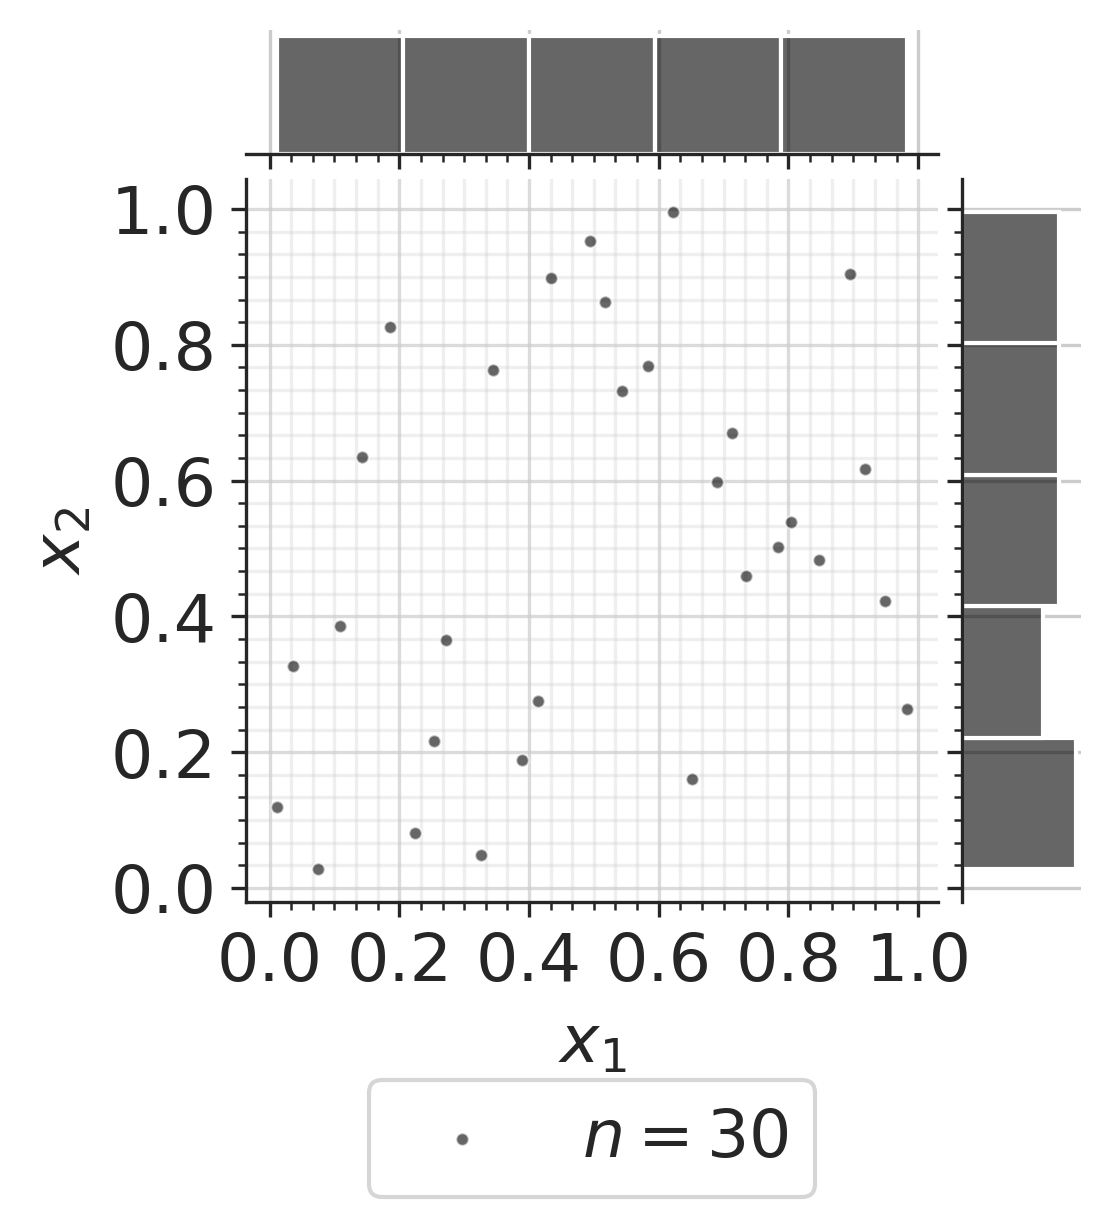
\includegraphics[width=\textwidth]{../numerical_experiments/chapter1/figures/poor_LHS.png}
        \caption{Poorly space-filling LHS}
    \end{subfigure}
    \hfill
    \begin{subfigure}[b]{0.32\textwidth}
        \centering
        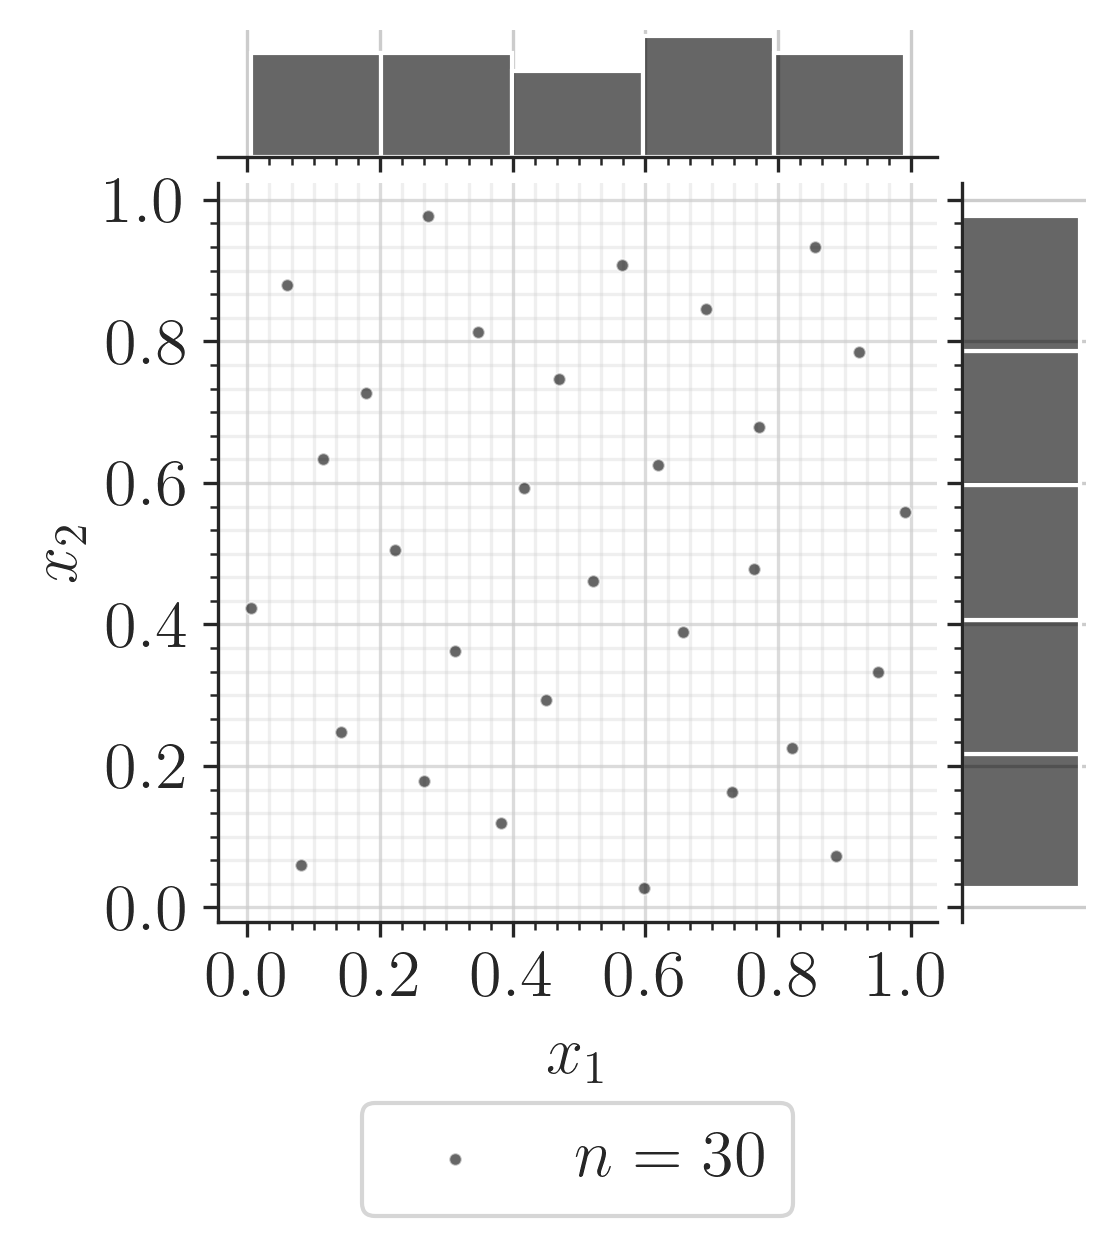
\includegraphics[width=\textwidth]{../numerical_experiments/chapter1/figures/optimized_C2_LHS.png}
        \caption{$L_2$ centered optimized LHS}
    \end{subfigure}
    \hfill
    \begin{subfigure}[b]{0.32\textwidth}
        \centering
        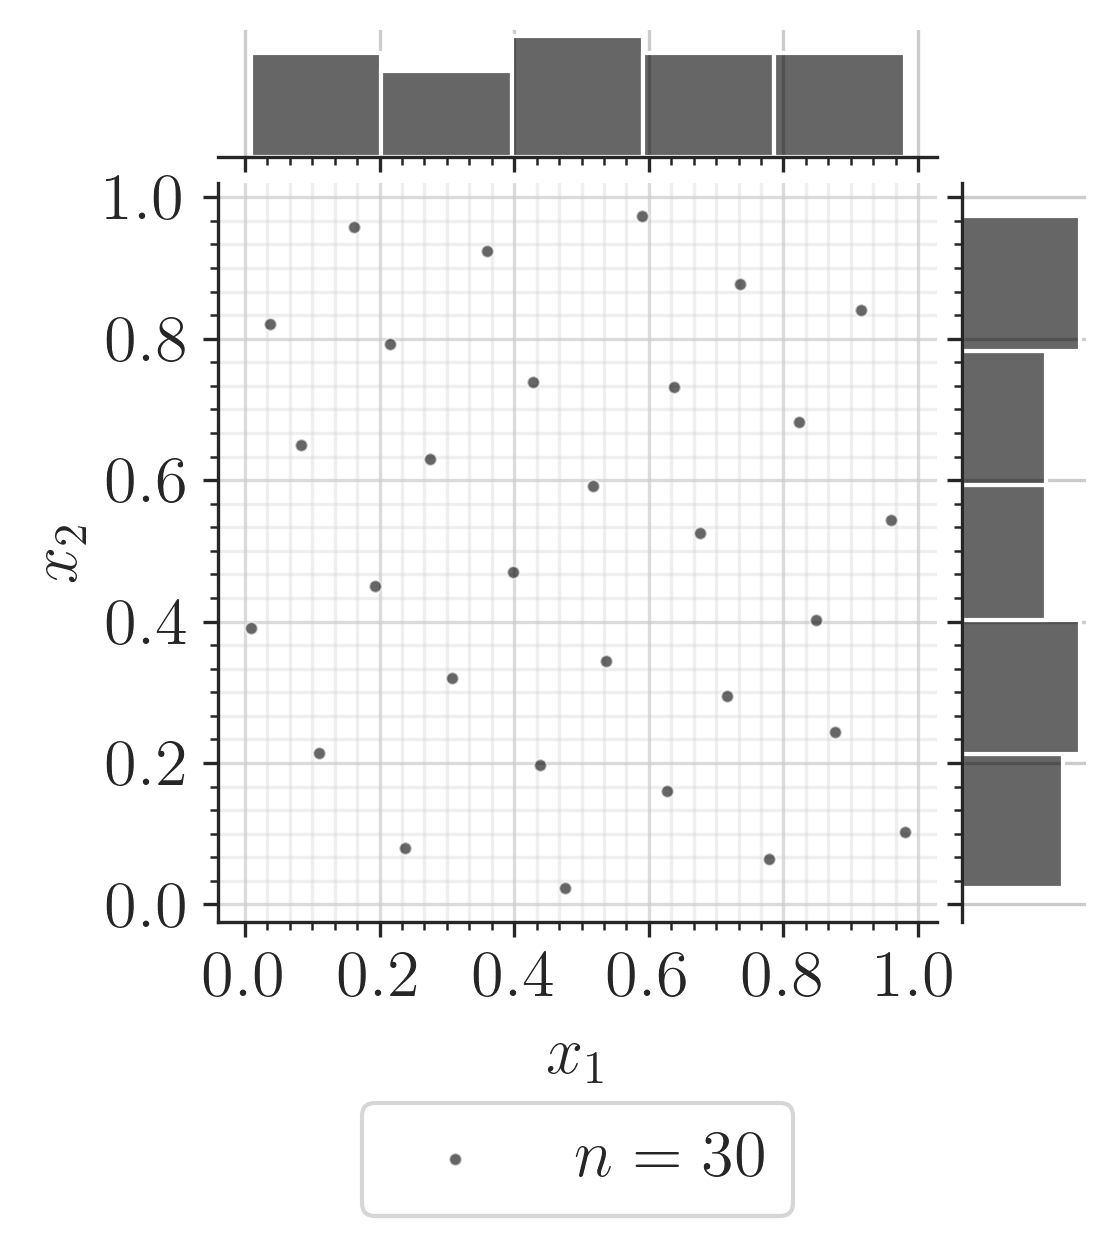
\includegraphics[width=\textwidth]{../numerical_experiments/chapter1/figures/optimized_phip_LHS.png}
        \caption{$\phi_p$ optimized LHS}
    \end{subfigure}
       \caption{Latin hypercube designs with poor and optimized space-filling properties ($n=8$)}
       \label{fig:LHS_designs}
\end{figure}

%============================================================%
\subsection{Summary and discussion}
%============================================================%


A wide panel of sampling techniques exists for numerical integration or design of experiments purposes. 
In both cases, the studied domain was bounded and the targeted measure was uniform. 
However, uncertainty propagation is often performed on complex input distributions, with possibly unbounded domains. 
In uncertainty quantification, this step might be referred to as the estimation of the output random variable's central tendency (i.e., its mean and variance).
Central tendency estimation is a numerical integration with respect to any input distribution, also named \textit{probabilistic integration} by \citet{briol_oates_2019}.  

To generate i.i.d samples following any distribution (i.e., non-uniform), one may use \textit{inverse transform} sampling.
This method first generates a sample in the unit hypercube, then, the inverse CDF function (i.e., quantile function) is applied on marginals. 
Finally, possible dependence effects can be added using the Sklar theorem \eq{thm:sklar}.

One may wonder if the properties from the uniform design are conserved after this nonlinear transformation. 
\citet{hickernell_2020} explores this question from a discrepancy point of view. 
The authors find correspondences between discrepancies with respect to uniformity and discrepancy with respect to the target distribution. 
However this result show practical limits, sometimes making the interpretation of the last discrepancy easier. 
This question will be further discussed using a more general framework in the \elias{Chapter xx}.

Let us also remark that, depending on the distribution, defining the inverse CDF is not always possible.
For example, samples following truncated distributions or mixture distributions might sometime be generated with a different technique. 
The \textit{acceptance-rejection} method offers a versatile generation only based on the PDF $f_{\bx}$.
Assuming that a well-known proposal PDF $f^*_{\bx}$ exists such that $f_{\bx} \leq c \times f^*_{\bx}, c \in [1, +\infty]$. 
Then, one may generate a sample according to $c \times f^*_{\bx}$ and only retain from this sample the points under the PDF $f_{\bx}$.
\elias{add illustration with truncated normal and triangular.}
Note that QMC sampling is not well suited with acceptance-rejection since its structure gets perturbed. 

\begin{itemize}
    \item \elias{Markov Chain Monte Carlo: when it is hard to sample from the distribution.}
    \item \elias{Add the summary table with the properties of each methods?}
\end{itemize}

In this section, many methods were presented to propagate input uncertainties against a deterministic function.
The propagation with the three following goals and contexts were introduced: 
\begin{itemize}
    \item building a quadrature rule for numerical integration against a uniform distribution,
    \item creating a space-filling design of experiments to uniformly explore the space, often in a small data context (e.g., to build the learning set of a surrogate model),
    \item generating a design for central-tendency estimation, which is simply a numerical integration against a non uniform density.
\end{itemize} 
%Note that some of these methods can also find a use in the context of data compression or quantization.
These three objectives have been explored in different communities but actually mostly share similar methods. 
They all have in common the general analysis (i.e., global behavior) of the output random variable. 
However, some studies require to shift the focus on specific areas of the output random variables.
When using uncertainty propagation to perform a risk analysis, the events studied are often contained in the tails of the output distribution. 
In this case, dedicated uncertainty propagation methods will significantly improve the estimation of the associated statistical quantities.


%============================================================%
%============================================================%
\section{Reliability-oriented uncertainty propagation}
%============================================================%
%============================================================%

This section aims at presenting another type of uncertainty propagation. 
In the context of a risk analysis applied to the engineering field, the reliability of a system needs to be assessed. 
Most often, a risk measure associated with a failure mode of the studied system is estimated. 

Since most systems studied in risk analysis should be highly reliable, the occurrence of such event is qualified as rare. 
Only an unlikely small amount of extreme input conditions or an unlikely unfavorable combinations of inputs lead to the failure of the system. 
Hence the usage of the equivalent terms \textit{reliability analysis} and \textit{rare event estimation}. 
The notion of risk associated with an event is often decomposed as a product of likelihood and impact. 
The failure of a system might be very rare but its consequences can be severe (e.g., civil engineering structures, nuclear infrastructure, telecommunication networks, electrical grid, railway signalling, etc.).

Different risk measures (i.e., quantities of interest) can be studied depending on the type of risk analysis. 
Quantiles are a first conservative measure, widely used for risk analysis. 
The $\alpha$-quantile $q_\alpha$ of the output random variable $Y$ is defined as:
\begin{equation}
    q_\alpha = \inf_{y\in\R}{\left\{F_Y(y) \geq \alpha\right\}}, \quad \alpha \in [0, 1].    
\end{equation}
\elias{define superquantiles in text?}
As an alternative, one can define a scalar safety threshold $\yth$ that should not be exceeded to keep the system safe. 
Then, a second risk measure is probability of exceeding this safety threshold, also called \textit{failure probability}: 
\begin{equation}
    \pf = \P\left(Y \geq \yth\right), \quad \yth\in\R.
\end{equation}
To illustrate this quantity, \fig{fig:1D_reliability} shows the one-dimensional propagation of a normal distribution (represented by the PDF on the left), throught a function $g(\cdot)$.
The probability of exceeding a given threshold $\yth$ is represented by the area in red under the output PDF on top.
An interesting reflection on the use and the interpretation of risk measures
\footnote{Including measures from the finance domain such as the \textit{conditional value-at-risk} (also called superquantile).} 
is presented in \citet{rockafellar_2015}. 

\begin{figure}
    \centering
    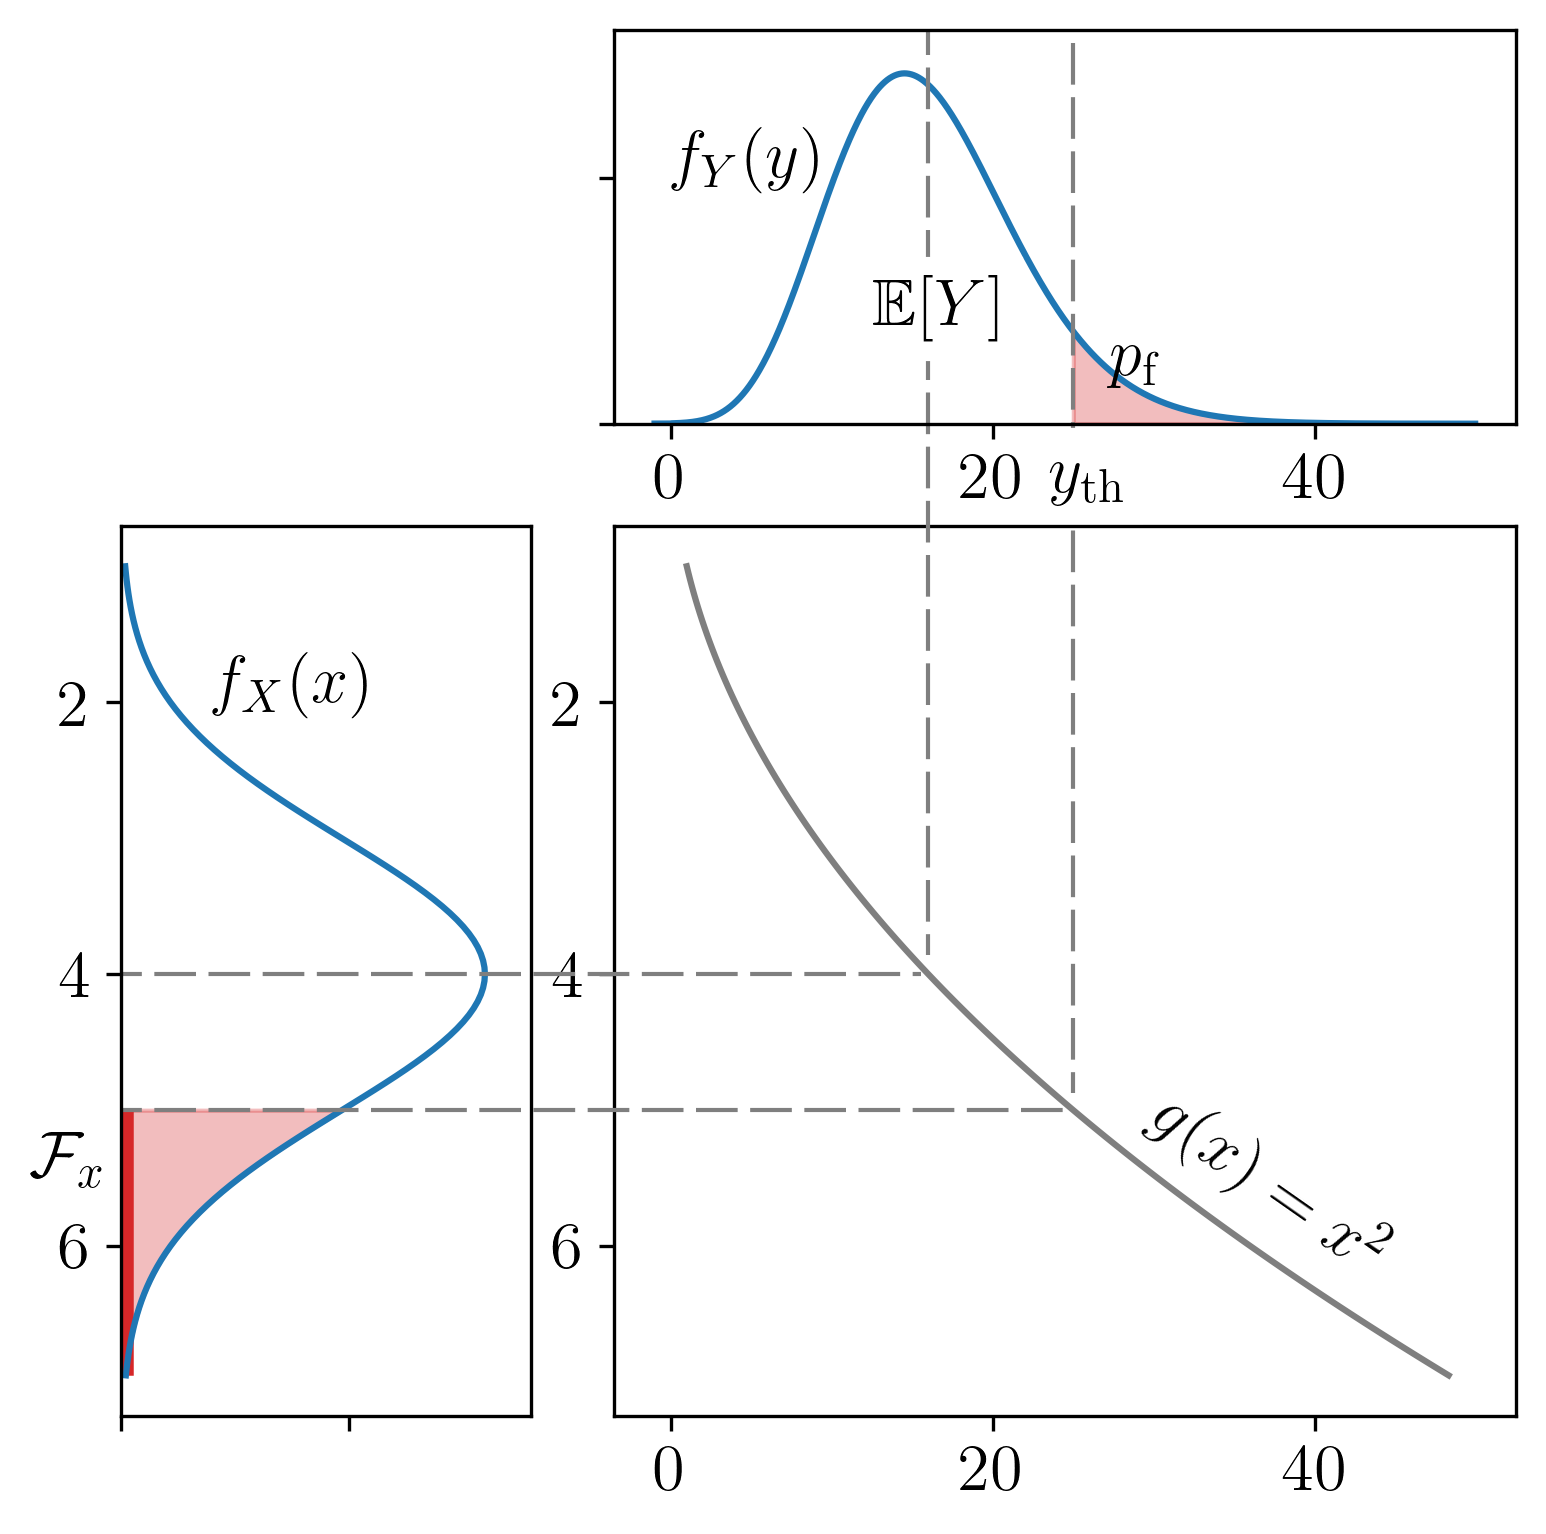
\includegraphics[width=0.5\textwidth]{../numerical_experiments/chapter1/figures/1D_reliability.png}
    \caption{One-dimensional reliability analysis example}
    \label{fig:1D_reliability}
\end{figure}

In the following, the formalism for reliability analysis problems will be first presented, 
then the main methods solving this specific problem will be introduced.
Note that the present work will not address the problems of time-dependent reliability analysis tackled in \citet{hawchar_2017}. 

%============================================================%
\subsection{Problem formalization}
%============================================================%

Following to the UQ methodology, the behavior of the system is modeled by $\iM(\cdot)$. 
Considering the problem of exceeding a safety threshold in \elias{add ref}, the system's performance is commonly defined as the difference between the model's output and a safety threshold $\yth\in\R$. 
Formally, the \textit{limit-state function} (LSF) is a deterministic function $g:\R\rightarrow\R$ quantifying this performance: 
\begin{equation}
    g(\bx) = \yth - \iM(\bx).
\end{equation}
Depending on the sign of its images, this function splits the inputs space into two disjoint and complementary domains called  
the \textit{failure domain} $\iF_{\bx}$, and the \textit{safe domain} $\mathcal{S}_\bx$ which are defined as:
\begin{equation}
    \iF_{\bx} = \{\bx \in \iD_\bx \, | \,  g(\bx) \leq \yth\}, \qquad 
    \mathcal{S}_\bx := \{\bx \in \iD_\bx \, | \, g(\bx) > \yth\}. 
    %\iD_\bx = \iF_{\bx} \cup \mathcal{S}_\bx 
\end{equation}
The border between these two domains is a hypersurface called \textit{limit-state surface} (LLS), defined by $\iF_{\bx}^0 := \{\bx \in \iD_\bx | g(\bx) = 0\}$.
Similarly to any UQ study around a numerical model, this problem ca require to be resolved using a limited numbers of calls to a black-box simulator.
The difficulties of a reliability problem might come from the properties of the LSF: nonlinear, costly to evaluate or with a multimodal failure domain. 
Additionally, note that the reliability problem can be the composition of multiple reliability problems, often modeled as system of problems in series and parallel.

A rare event estimation results from a particular uncertainty propagation through the LSF. 
Considering the resulting output variable of interest $g(\bX)$, its probability of being negative (i.e., in the failure domain) is a common risk measure \elias{add pointer}.
The commonly named \textit{failure probability}, denoted $\pf$, will be our quantity of interest in reliability analysis.
This quantity is formally written\footnote{Note that this probabilistic integration is usually written using the PDF $f_\bX(\cdot)$ 
but it could identically be expressed in terms of probability measure by taking $f_\bX(\bx) \, \dd\bx = \dd \mu(\bx), \, \forall \bx \in \iD_\bx$.}: 
\begin{equation}
    \begin{split}
        \pf := \P(Y \geq \yth) &= \P(g(\bX) \leq 0)\\
        &= \int_{\iF_\bx} f_\bX(\bx) \, \dd\bx
        = \int_{\iD_\bx} \1_{\iF_\bx}(\bx) f_\bX(\bx) \, \dd\bx,
    \end{split}
\end{equation}
were the indicator function applied to the failure domain returns $\1_{\left\{\iF_{\bX}\right\}}(x) = 1$ if $x \in \iF_{\bX}$ and $\1_{\left\{\iF_{\bX}\right\}}(x) = 0$ otherwise.
Rare event estimation implies both contour finding (i.e., characterizing the LSF) and an estimation strategy targeting the failure domain (often with a limited number of simulations).
Note that failure event are qualified as rare when its failure probability has an order of magnitude between $10^{-2} \leq \pf \leq 10^{-9}$ \elias{lemaire 2009}.

Instead of directly performing a reliability analysis in the physical space (i.e., $\bx$-space), these problems are usually solved in the \emph{standard normal space} (i.e., $\bu$-space).
Worsting in the standard space reduces numerical issues potentially caused by unscaled or asymmetric marginals. 
Moreover, a larger panel of methods can be applied in the standard space since the random inputs are independent.   
The bijective mapping between these two spaces is called an ``iso-probabilistic transformation'', 
denoted $T: \iD_{\bx} \subseteq \R^d \rightarrow \R^d, \bx \mapsto T(\bX) = \bu = \left(u_1, \dots, u_d\right)\TT$. 
When considering any random vector $\bX = \left(X_1, \dots, X_d\right)\TT$ and the independent standard Gaussian vector $\bU = \left(U_1, \dots, u_d\right)\TT$, the following equalities hold:
\begin{equation}
    \bU = T(\bX) \Leftrightarrow \bX = T^{-1}(\bU).
\end{equation} 

A reliability problem can be expressed in the standard normal space. 
Let us first consider the transformed limit-state function $\check{g}$ defined as: 
\begin{equation}
    \cg : \bigg|
    \begin{array}{rcl}
        \R^d & \longrightarrow & \R\\
        \bu & \longmapsto & \check{g}(\bu) = \left(g \circ T^{-1}\right)(\bu).
    \end{array}
\end{equation}

Since this transformation is a diffeomorphism\footnote{Considering two manifolds $A$ and $B$, a transformation $T: A \rightarrow B$ is called a diffeomorphism if it is a differentiable bijection with a differentiable inverse $T^{-1} : B \rightarrow A$.}, 
one can apply the change of variable $\bx = T(\bu)$ to express the realibility problem from \elias{add pointer} in the standard space: 
\begin{equation}
    \pf = \P(\cg(\bU) \leq 0) 
        = \int_{\iF_\bu} \varphi_d(\bu) \, \dd\bu 
        = \int_{\R^d} \1_{\iF_\bu}(\bu) \varphi_d(\bu) \, \dd\bu,
\end{equation}
with the transformed failure domain noted $\iF_\bu = \{\bu \in \R^d \, | \, \cg(\bu) \leq 0\}$, 
and the $d$-dimensional standard Gaussian PDF $\varphi_d(\bu) = \frac{1}{(2\pi)^{d/2}} \exp\left(-\frac{\lVert\bu\rVert^2_2}{2}\right)$. 
The fact that the failure probability is invariant by this transformation allows the analyst to estimate this quantity in both spaces.  

Different types of transformations exist, such as the Rosenblatt or the generalized Nataf transformation \citep{Lebrun_PHD_2013}
In practice, the transformation choice depends on the properties of the input distribution studied. 
\elias{When should we use what? In this case the distribution is not elliptical so the default method is the Rosenblatt transform.}



%============================================================%
\subsection{Rare event estimation methods}
%============================================================%
%\elias{Why are the previous sampling methods not suited for rare events?}
%\elias{Surrogate based methods can help the contour finding step.}

The main risk measure chosen for rare event estimation in this work is the previously introduced failure probability.
Therefore, let us recall that the goal is to build an efficient estimation (or approximation) of the following $d$-dimensional integral: 
\begin{equation}
    \pf = \int_{\iD_\bx} \1_{\iF_\bx}(\bx) f_\bX(\bx) \, \dd\bx
\end{equation}

In the context of rare event estimation using costly to evaluate numerical models, the simulation budget is often limited to $n$ runs with $\pf \ll \frac1n$. 
Which explains the need for specific methods offering approximations or simulations targeting the unknown failure domain. 
Two types of rare event estimation methods are classically presented: first, using approximation approaches, second, using sampling techniques. 
This section introduced the commonly used rare event methods, see \cite{MorioBalesdent2015} for a more exhaustive review.


%------------------------------------------------------------%
\subsubsection{First and second order reliability methods (FORM/SORM)}
%------------------------------------------------------------%

The so-called First and second order reliability methods (FORM and SORM) both rely on a geometric approximation to estimate a failure probability.
They extrapolate a local approximation of the LSF built in the vicinity of a \textit{most-probable-failure-point} (MPFP), also called \textit{design point}.
\elias{add some refs}


Working in the standard space, the methods first look for this MPFP, denoted $P^*$, with coordonates $\bu^*$, 
To find it, one can solve the following quadratic optimization problem: 
\begin{equation}
    \bu^* = \argmax_{\bu \in \R^d} \left(\1_{\iF_\bu}(\bu) \varphi_d(\bu)\right).
\end{equation}
Using the properties of the standard space allows us to rewrite it as: 
\begin{align}
    \bu^* &= \argmax_{\bu \in \R^d} \, \frac{1}{(2\pi)^{d/2}} \exp\left(-\frac{\bu\TT \bu }{2} \right) \qquad \mathrm{s.t.} \quad \bu \in \iF_{\bu}\\
          &= \argmin_{\bu \in \R^d} \, \bu\TT \bu \qquad \mathrm{s.t.} \quad \cg(\bu) \leq 0.
\end{align}
This problem becomes a quadratic optimization under nonlinear constraint. 
It is classically solved by gradient decent algorithms (e.g., AbdoRackwitz algorithm \elias{add ref}) but can also use gradient-free techniques (e.g., Cobyla algorithm \elias{add ref}).
This point (assuming that it is unique) defines the smallest Euclidian distance between the LSS and the origin of the standard space.
To understand its role in the reliability problem, let us recall that the density of the standard normal present an exponential decay in its radial and tangential direction.
Then, $P^*$ is the point with the biggest contribution to the failure probability \elias{pointer}. 

This distance between the origin and $P^*$ is a different risk measure, introduced as the \textit{Hasofer-Lind reliability index} \elias{add ref}, $\beta \in \R$ such that:
\begin{equation}
    \beta = \Vert \bu^* \Vert_2 = \balpha \TT \bu^*, \qquad \mathrm{s.t.} \quad
        \balpha = \frac{\nabla_{\bu} \,  \cg(\bu)}{\Vert \nabla_{\bu} \,  \cg(\bu) \Vert_2}.      
    %= \min_{\cg(\bu)=0} \left(sqrt{\bu\TT\bu}\right)
\end{equation}
The vector $\balpha$ is the unit vector pointing at $P^*$ from the origin point. 

Then, FORM aims at approximating the limit-state function $\cg(\cdot)$ by its first-order Taylor expansion around the MPFP, denoted $\cg_1(\bu^*)$: 
\begin{equation}
    \begin{split}
        \cg(\bu) &= \cg_1(\bu^*) + o\left(\Vert \bu - \bu^* \Vert_2^2\right)\\
                 &= \cancel{\cg(\bu^*)} + \nabla_{\bu} \,  \cg(\bu^*)\TT \left(\bu -\bu^* \right) + o\left(\Vert \bu - \bu^* \Vert_2^2\right)\\
                 &= \Vert \nabla_{\bu} \, \cg(\bu) \Vert_2 \left(\balpha\TT \bu^* - \balpha\TT \bu \right) + o\left(\Vert \bu - \bu^* \Vert_2^2\right)
    \end{split}    
\end{equation}
 
Using $\cg_1(\cdot)$ as approximation of the LSF, the failure probability can be approximated as: 
\begin{equation}
    \pf \approx \pf^{\mathrm{FORM}} = \P\left(- \balpha\TT \bu \leq -\beta\right) = \Phi(-\beta),
\end{equation} 
with $\Phi(\cdot)$ the CDF of the standard Gaussian. 
Depending on the properties of the LFS, this approximation will be more or less accurate. 
Note that for a linear LFS, $\pf = \pf^{\mathrm{FORM}}$. 
When the function is nonlinear, adding a quadratic term to the Taylor expansion can help the approximation. 
The approximation method is then called SORM for \textit{second order reliability method}. 
However, this added complexity implies the computation of Hessian matrices, which can be complicated (see \elias{Bourinet Chap. 1 for their estimation}).


\begin{figure}[ht]
    \centering
    \begin{subfigure}[b]{0.32\textwidth}
        \centering
        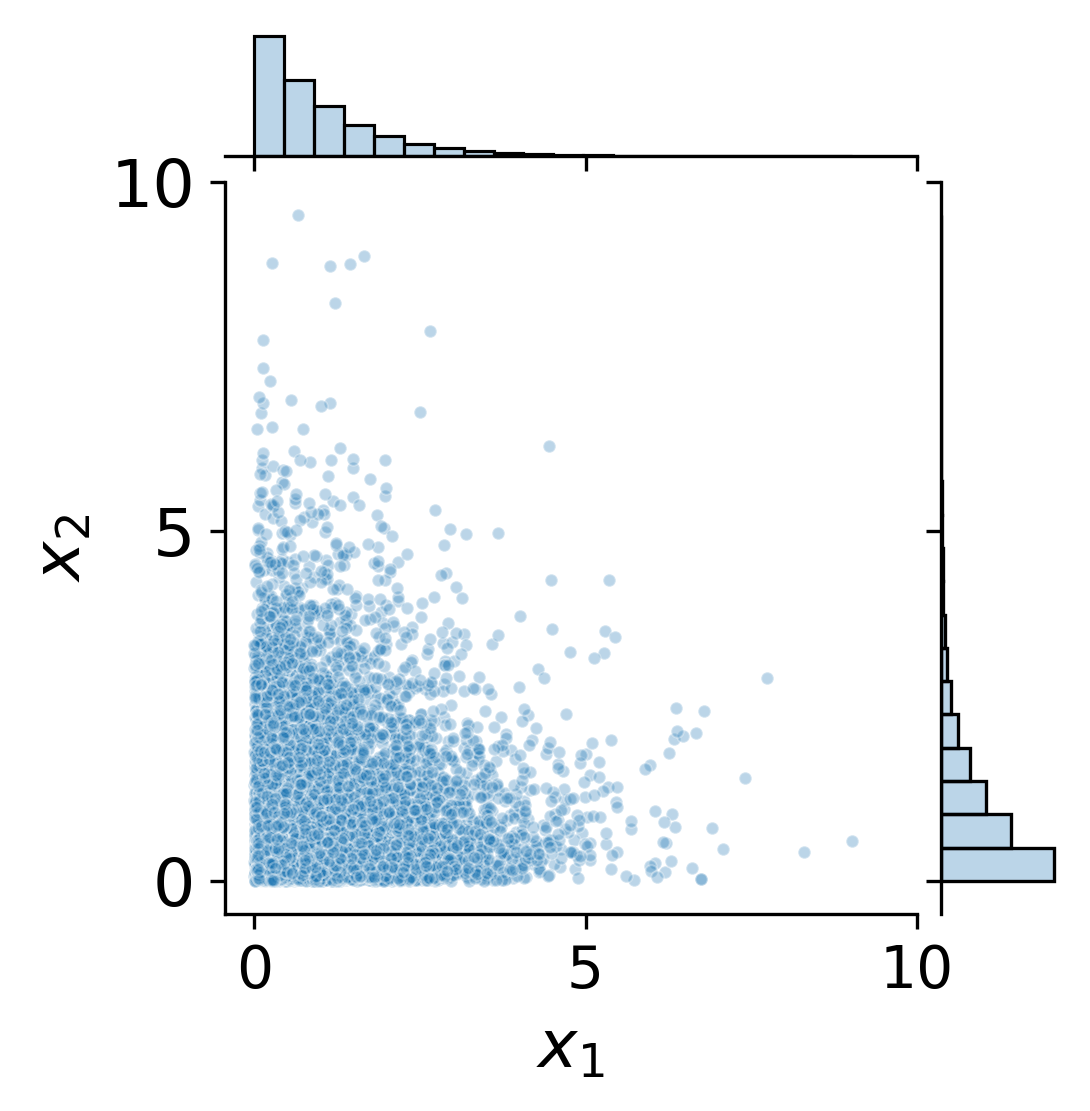
\includegraphics[width=\textwidth, draft]{../numerical_experiments/chapter1/figures/independent_copula.png}
        \caption{FORM approximation}
    \end{subfigure}
    \quad
    \begin{subfigure}[b]{0.32\textwidth}
        \centering
        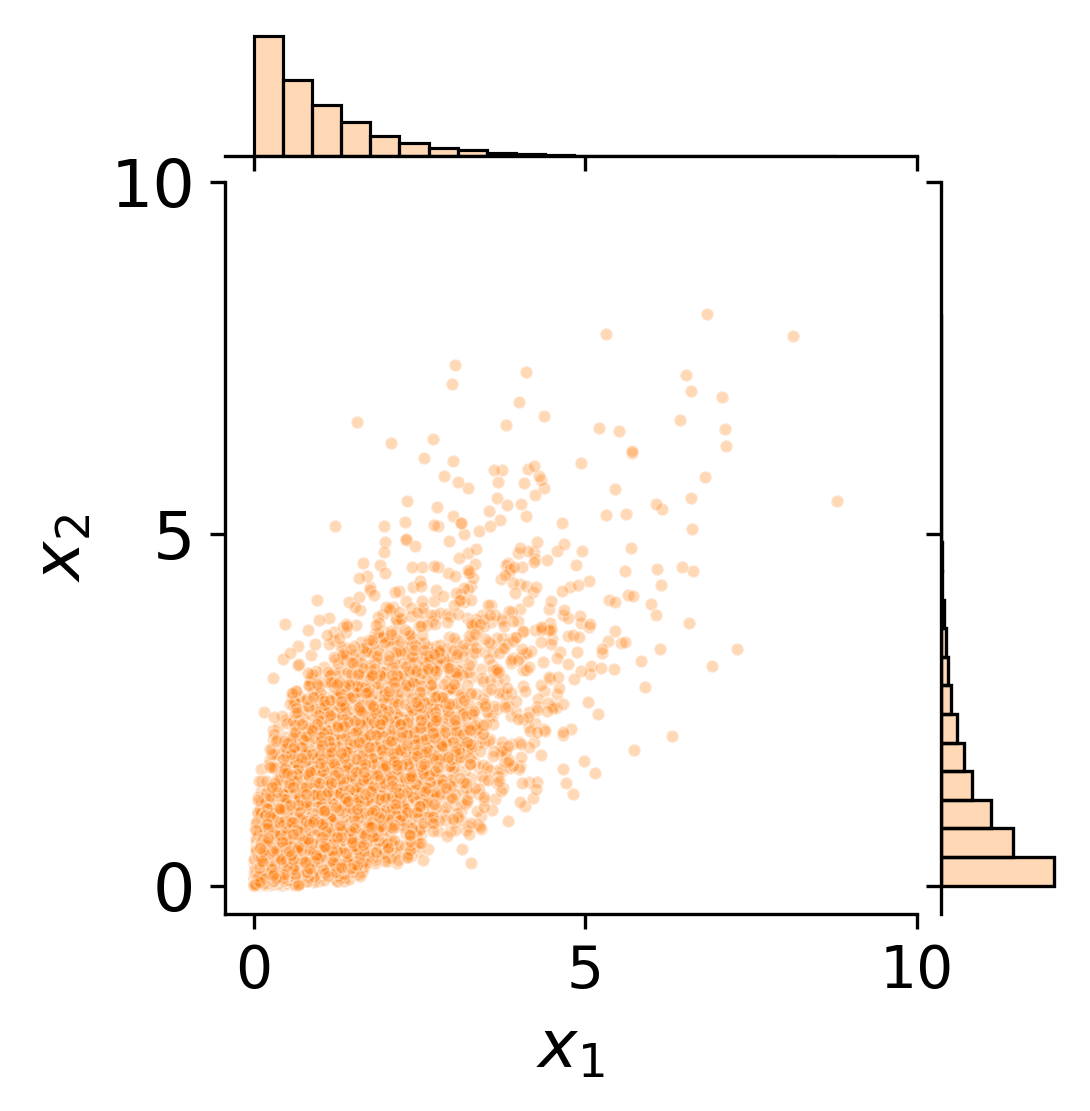
\includegraphics[width=\textwidth, draft]{../numerical_experiments/chapter1/figures/normal_copula.png}
        \caption{SORM approximation}
    \end{subfigure}
       \caption{FORM and SORM approximation on a two-dimensional example}
       \label{fig:FORM_SORM_approx}
\end{figure}


When the MPFP is not unique, the application of these methods might lead to important errors.
From a geometrical point of view, having more than one MPFP means that more than one failure zones are at the same euclidean distance of the origin.
Applying a FORM or SORM resolution in this particular case leads to the estimation of only one of the failure zones.
The \textit{muti-FORM} algorithm developed by \elias{add ref} prevents this situation by applying successive FORM. 
Once the first MPFP $P^{*^{(1)}}$ found, the LSS is modified by removing a nudge to find to following MPFP $P^{*^{(2)}}$. 

\begin{figure}[ht]
    \centering
    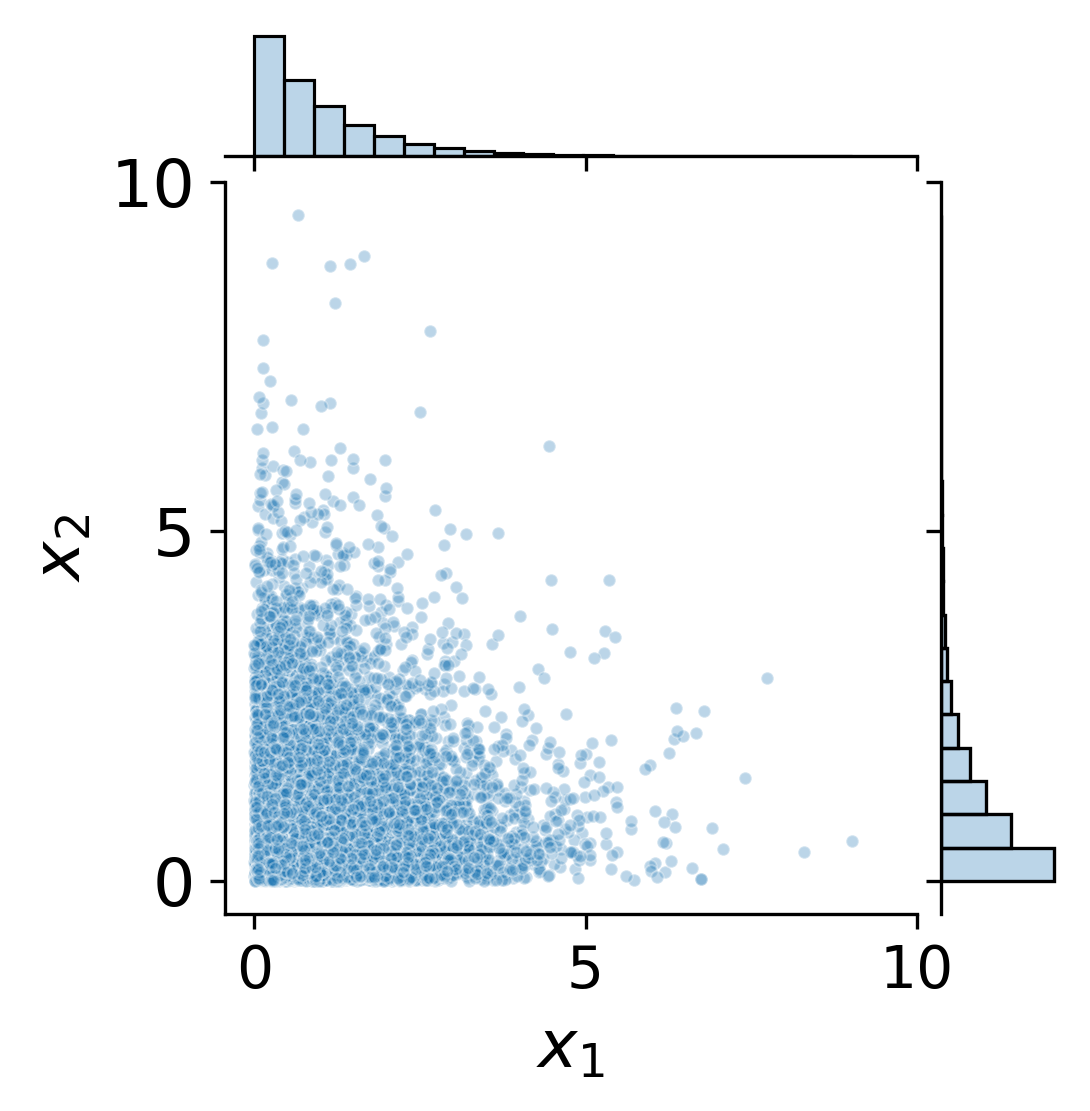
\includegraphics[width=0.32\textwidth, draft]{../numerical_experiments/chapter1/figures/independent_copula.png}
    \caption{Multi-FORM approximation on an example with two MPFPs}
    \label{fig:multi_FORM}
\end{figure}

%FORM/SORM first looks for an appropriate approximation of the limit state surface by a simple hypersurface. 
%Then, working in the standard space allows direct calculation of the failure probability considering the approximated limit state function.

Overall, FORM and SORM methods deliver a very efficient approximation of small probabilities for relatively simple problems (in terms of linearity and dimension). 
For this reason, they have been widely used in the practical context of limited simulation budget. 
However, these methods present serious limits as the dimension increases (see the discussion in \elias{Chabridon} Chapt. 1). 
Additionally, their main drawback is the lack of complementary information concerning the confidence of the results. 
The example from the \elias{Fig xx} has shown that the method might miss some important areas of the failure domain, leading to poor estimations. 
As an alternative to approximation methods, simulation-based methods often provide to the analyst an assessment of the estimation's confidence. 



%------------------------------------------------------------%
\subsubsection{Monte Carlo}
%------------------------------------------------------------%
Crude Monte Carlo sampling is a universal and empirical method for uncertainty propagation. 
As introduced earlier, it relies on the pseudo-random generation of a i.i.d. sample $\left\{\bx^{(i)}\right\}_{i=1}^n \simiid f_\bX$.   
Only the estimator is written using the indicator function with the LSF: 
\begin{equation}
    \pf \approx \what{\pf}^{\textrm{MC}} = \frac1n \sum_{i=1}^{n} \1_{\iF_\bx}(\bx^{(i)})
\end{equation} 

Provided that the failure probability is bounded, this estimator converges towards it almost surely according to the LLN. 
Once again, Monte Carlo offers a nonbaised estimator, regardless of the problem's dimension or regularity of the function $g(\cdot)$  
Additionally, the variance of this estimator is fully known:
\begin{equation}
    \var\left(\what{\pf}^{\textrm{MC}}\right) = \frac1n \pf (1 - pf)
\end{equation} 
The variance of this estimator can be used to build its confidence interval according to the TCL \elias{pointer to the previous IC}. 
Because of the small scale of the quantities manipulated in rare event estimation, the estimator's coefficient of variation is also widely used: 
\begin{equation}
    \delta_{\what{\pf}^{\textrm{MC}}} = \frac{\sqrt{\var\left(\what{\pf}^{\textrm{MC}}\right)}}{\E[\what{\pf}^{\textrm{MC}}]}
                                      = \sqrt{\frac{1 - \pf}{n \pf}}.
\end{equation}

On paper, Monte Carlo estimator presents multiple advantages for rare event estimation.
First, this method can be applied directly in the physical space, without transformation (which is practical for complex input distributions).
Second, it does not suffer from the curse of dimensionality. 
Thrid, it is qualified as embarrassingly parallel method since each numerical simulations are independent.
Finally, it offers strong convergence guaranties and complementary information on the estimation confidence.
\elias{These properties make it the reference method.}


However, these advantages of this estimator are shadowed by its slow convergence. 
To estimate a target failure probability $\pf=10^{-\alpha}$, 
a Monte Carlo estimation with a convergence level $\delta_{\what{\pf}^{\textrm{MC}}} = 0.1$ famously requires $n=10^{\alpha + 2}$ simulations. 

In the context of rare event estimation, Monte Carlo needs a number of simulation that is often prohibitive in practice. 
This excessive simulation budget comes from the fact that the vast majority of the samples drawn from the input distribution are not in the failure domain.


\newpage
%------------------------------------------------------------%
\subsubsection{Importance sampling}
%------------------------------------------------------------%

Importance sampling (IS) is a variance reduction method, aiming at improving the performances of crude Monte Carlo sampling. 
In the context of rare event estimation, the main idea is to deliberately introduce a bias in the sampled density, shifting it towards the failure domain. 
If this shift actually goes towards the failure domain, it allows to draw more points in it, leading to a better estimate of our quantity.

The challenge in importance sampling is to pick a relevant \textit{instrumental} distribution $h_\bX$ (also called \textit{auxiliary} distribution) to replace the distribution $f_\bX$. 
Then, by introducing the fully known likelihood ratio $w_\bX(\bx) = \frac{f_\bX(\bx)}{h_\bX(\bx)}$, one can rewrite $f_\bX(\bx) = w_\bX(\bx) h_\bX(\bx)$ and inject it in the failure probability expression: 
\begin{equation}
    \pf = \int_{\iD_\bx} \1_{\iF_\bx}(\bx) f_\bX(\bx) \, \dd\bx
        = \int_{\iD_\bx} \1_{\iF_\bx}(\bx) w_\bX(\bx) h_\bX(\bx) \, \dd\bx
\end{equation}
This simple writing trick allows us to integrate against the auxiliary distribution. 
With a Monte Carlo method, this task should be easier than integrating directly against the initial distribution.

The importance sampling estimator of the failure probability is defined for a sample drawn on the auxiliary distribution $\left\{\bx^{(i)}\right\}_{i=1}^n \simiid h_\bX$: 
\begin{equation}
    \what{\pf}^{\mathrm{IS}} = \frac1n \sum_{i=1}^{n} \1_{\iF_\bx}(\bx^{(i)}) w_\bX(\bx^{(i)}).
\end{equation}
This estimator is unbiased and its variance is defined as: 
\begin{equation}
    \var\left( \what{\pf}^{\mathrm{IS}}\right) = \frac1n \left( \E_{h_\bX}\left[\left(\1_{\iF_\bx}(\bX) w_\bX(\bX)\right)^2\right] - \pf^2\right).
\end{equation}
The quality of the variance reduction in this method fully depends on the choice of the instrumental distribution. 
An optimal instrumental distribution $h_{\bX}^*$ theoretically gives the smallest variance by setting it equal to zero in \elias{pointer}: 
\begin{equation}
    h_{\bX}^*(\bx) = \frac{\1_{\iF_\bx}(\bx) f_\bX(\bx)}{\pf}. 
\end{equation}
This optimal results presented in \elias{add ref} is unfortunately not usable in practice since it uses the targeted quantity $\pf$. 
Knowing this framework, various techniques try to define instrumental distributions as close as possible to this theoretical result. 
Three main importance sampling techniques are used in this work. 

\elias{First, FORM-iS}

\elias{Second AIS-CE} 

\elias{Finally, NAIS}
 
Appendix \ref{apx:C} develops an algorithmic presentation of the two last techiniques: NAIS and AIS-CE.

\elias{Discussion on commun advantages and drawback of the IS methods.}

%------------------------------------------------------------%
\subsubsection{Subset sampling}
%------------------------------------------------------------%

Subset sampling splits the failure event $\iF_{\bx}$ into an intersection of $k_\#$ intermediary events $\iF_{\bx} = \cap_{k=1}^{k_\#} \iF_{[k]}$.
Each are nested such that $\iF_{[1]} \supset \dots \supset \iF_{[k_\#]} = \iF_{\bx}$.
The failure probability is then expressed as a product of conditional probabilities:
\begin{equation}
    \pf = \P(\iF_{\bx}) = \P(\cap_{k=1}^{k_\#} \iF_{[k]}) = \prod_{k=1}^{k_\#} \P(\iF_{[k]} | \iF_{[k-1]}).
\end{equation}
From a practical point of view, the analyst tunes the algorithm by setting the intermediary probabilities $\P(\iF_{[k]} | \iF_{[k-1]}) = p_0, \forall k \in \{1, \dots, k_\# \}$. 
Then, the corresponding quantiles $q_{[1]}^{p_0} > \dots > q_{[k_\#]}^{p_0}$ are estimated for each conditional subset samples $\bX_{[k], N}$ of size $N$. 
Note that the initial quantile is estimated by crude Monte Carlo sampling on the input PDF $f_{\bX}$. 
Following conditional subset samples are generated by MCMC sampling of $f_{\bX}(\bx |\iF_{[k-1]})$, using as seeds initialisation points the $n= N p_0$ samples given by $\mathbf{A}_{[k], n}=\{\bX_{[k-1]}^{(j)} \subset \bX_{[k-1], N}| g(\bX_{[k-1]}^{(j)}) > \widehat{q}_{[k-1]}^\alpha \}_{j=1}^n$. 
This process is repeated until an intermediary quantile exceeds the threshold: $\widehat{q}_{[k_\#]}^{p_0} < \yth$. 
Finally, the failure probability is estimated by:
\begin{equation}
    \pf \approx \widehat{\pf}^{\mathrm{SS}} = p_0^{k_\# -1} \frac1N \sum_{j=1}^N \1_{\{g(\bx) \leq \yth\}} (\bX_{[k_\#],N}^{(j)}).
\end{equation}

In practice, the subset sample size should be large enough to properly estimate intermediary quantiles, which leads \cite{AuBeck2001} to recommend setting $p_0=0.1$. 
SS efficiency depends on the proper choice and tuning of the MCMC algorithm \citep{Papaioannou_PEM_2015}. 
%Our work uses the SS implementation from \texttt{OpenTURNS}\footnote{\href{https://openturns.github.io/www/index.html}{https://openturns.github.io/www/index.html}} \citep{baudin_dutfoy_2017} which integrates a component-wise Metropolis-Hastings algorithm. 
%As an alternative to generating samples on a conditional distribution by MCMC, one could try to fit this conditional distribution.





\elias{Mention the appendix Appendix \ref{apx:C} presenting the algorithms of SS}


\elias{Discussion: Which strategy to solve these problems?}



%============================================================%
%============================================================%
\section{Sensitivity analysis}
%============================================================%
%============================================================%

%============================================================%
\subsection{Global sensitivity analysis}
%============================================================%

%============================================================%
\subsection{Reliability-oriented sensitivity analysis}
%============================================================%





%============================================================%
%============================================================%
\section{Metamodeling}
%============================================================%
%============================================================%
Note that the calibration error is often larger than the metamodeling error.

%============================================================%
\subsection{Global metamodel}
%============================================================%

%============================================================%
\subsection{Contour finding for rare-event estimation}
%============================================================%






%============================================================%
%============================================================%
\section{Conclusion}
%============================================================%
%============================================================%
